\documentclass{beamer}

\usepackage{default}
\usepackage[utf8]{inputenc}

\usepackage{graphicx}
\usepackage{hyperref}
\usepackage{nameref}
\usepackage{amsthm}
\usepackage{amsmath}
\usepackage{amssymb}
\usepackage{bm,array}
\usepackage{algorithm}
\usepackage{multirow}
\usepackage{subcaption}
\usepackage[noend]{algpseudocode}
\usepackage{pifont}
\usepackage{lipsum}
\usepackage{tikz}
\usetikzlibrary{shapes,arrows,decorations,shapes}
\usetikzlibrary{arrows.meta}
\usetikzlibrary{decorations.pathreplacing} 

\author{João Valença\\valenca@student.dei.uc.pt}
\institute{Department of Informatics Engineering\\University of Coimbra}
\date{February 2, 2015}
\subject{Theoretical Computer Science}
\title{Visualisation and Analysis of Geographic Information}
\subtitle{Algorithms and Data Structures}

\setbeamertemplate{navigation symbols}{}
\addtobeamertemplate{navigation symbols}{}{%
	\usebeamerfont{footline}%
	\usebeamercolor[fg]{footline}%
	\hspace{1em}%
	-- \insertframenumber\ --
}

\newcommand{\smark}{\ding{110}}%
\newcommand{\cmark}{\ding{108}}%
\newcommand{\tmark}{\ding{115}}%

\begin{document}
\frame{
	\titlepage
}
\frame{
	\frametitle{Motivation}
	\begin{itemize}
		\item Reduce visual information when displaying large numbers of geographic points
		\item Find a representative subset of a collection of geographic points
		\begin{figure}[H]
	\centering
	\begin{minipage}{0.4\linewidth}
		\centering
		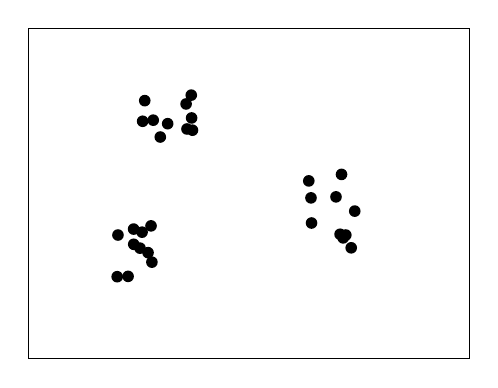
\begin{tikzpicture}[scale=1.4]
			\draw (-0.5,-0.4) rectangle (3.5,2.6);
			
			\fill (0.456,0.778)circle (1.5pt);
			\fill (0.622,0.478)circle (1.5pt);
			\fill (0.457,0.64)circle (1.5pt);
			\fill (0.614,0.807)circle (1.5pt);
			\fill (0.314,0.724)circle (1.5pt);
			\fill (0.533,0.75)circle (1.5pt);
			\fill (0.514,0.605)circle (1.5pt);
			\fill (0.307,0.346)circle (1.5pt);
			\fill (0.406,0.349)circle (1.5pt);
			\fill (0.587,0.564)circle (1.5pt);
			
			\fill (2.065,1.061)circle (1.5pt);
			\fill (2.045,1.215)circle (1.5pt);
			\fill (2.292,1.07)circle (1.5pt);
			\fill (2.381,0.724)circle (1.5pt);
			\fill (2.43,0.608)circle (1.5pt);
			\fill (2.342,1.274)circle (1.5pt);
			\fill (2.329,0.731)circle (1.5pt);
			\fill (2.462,0.941)circle (1.5pt);
			\fill (2.357,0.698)circle (1.5pt);
			\fill (2.07,0.833)circle (1.5pt);
			
			\fill (0.765,1.734)circle (1.5pt);
			\fill (0.557,1.943)circle (1.5pt);
			\fill (0.698,1.613)circle (1.5pt);
			\fill (0.634,1.766)circle (1.5pt);
			\fill (0.979,1.993)circle (1.5pt);
			\fill (0.99 ,1.675)circle (1.5pt);
			\fill (0.538,1.756)circle (1.5pt);
			\fill (0.932,1.913)circle (1.5pt);
			\fill (0.982,1.786)circle (1.5pt);
			\fill (0.94 ,1.686)circle (1.5pt);
		\end{tikzpicture}
		\caption*{\footnotesize Original Set}
		\label{fig:badrep}
	\end{minipage}
	\hspace{1cm}
	\begin{minipage}{0.4\linewidth}
		\centering
		\begin{tikzpicture}[scale=1.4]
		\draw (-0.5,-0.4) rectangle (3.5,2.6);
		
		\fill (0.765,1.734)circle (1.5pt);
		\fill (0.514,0.605)circle (1.5pt);
		\fill (2.292,1.07)circle (1.5pt);
		\end{tikzpicture}		
		\caption*{\footnotesize Representative Subset}
		\label{fig:goodrep}
	\end{minipage}
	\caption{Example of a Representative Set}
	\label{fig:rep}
\end{figure}
	\end{itemize}
	
}

\frame{
	\frametitle{Coverage}	
	\begin{itemize}
		\item Minimising Coverage
	\end{itemize}
	\begin{figure}[H]
	\centering
	\begin{minipage}{0.45\linewidth}
		\centering
		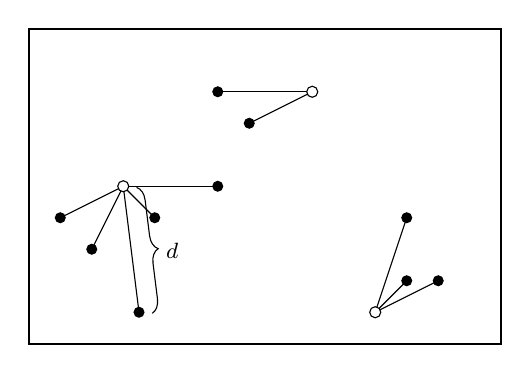
\begin{tikzpicture}[scale=0.4]
		
		\draw [<->,thick] (0,0) rectangle (15,10) {};
		%centroids
		
		%Left Group
%		\fill ( 7,7) circle (5pt);
		\fill ( 1,4) circle (5pt);
		\fill ( 4,4) circle (5pt);
		\fill ( 2,3) circle (5pt);
		\fill (3.5,1) circle (5pt);
		\fill ( 6,5) circle (5pt);
		
		%Middle Group
		
		\fill ( 7,7) circle (5pt);
		\fill ( 6,8) circle (5pt);
		
		%Right Group
		\fill (12,2) circle (5pt);
		\fill (12,4) circle (5pt);
		\fill (13,2) circle (5pt);
		
		%Lines
		\draw [-] (1,4) -- (3,5);
		\draw [-] (4,4) -- (3,5);
		\draw [-] (2,3) -- (3,5);
		\draw [-] (3.5,1) -- (3,5);
		\draw [-] (6,5) -- (3,5);
		
		\draw [-] (7,7) -- (9,8);
		\draw [-] (6,8) -- (9,8);
		
		\draw [-] (12,2) -- (11,1);
		\draw [-] (12,4) -- (11,1);
		\draw [-] (13,2) -- (11,1);
		\fill [white] (11,1) circle (5pt);
		\fill [white] ( 3,5) circle (5pt);
		\fill [white] ( 9,8) circle (5pt);
		
		\draw (11,1) circle (5pt);
		\draw ( 3,5) circle (5pt);
		\draw ( 9,8) circle (5pt);
		
		\draw [decorate,decoration={brace,amplitude=5pt},xshift=12pt,yshift=-1pt]
		(3,5) -- (3.5,1)node [black,midway,xshift=10pt] {\footnotesize$d$};
		\end{tikzpicture}
		\caption*{Non-Optimal Assignment}
		\label{fig:badcov}
	\end{minipage}
	\begin{minipage}{0.45\linewidth}
		\centering
		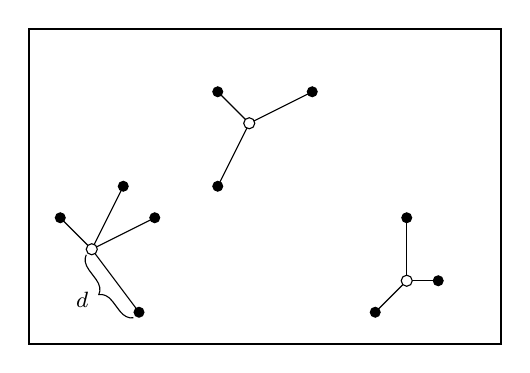
\begin{tikzpicture}[scale=0.4]
		
		\draw [<->,thick] (0,0) rectangle (15,10) {};
		%centroids
		
		%Left Group
		\fill ( 1,4) circle (5pt);
		\fill ( 4,4) circle (5pt);
		\fill ( 3,5) circle (5pt);
		\fill (3.5,1) circle (5pt);
		
		%Middle Group
		\fill ( 6,5) circle (5pt);
		\fill ( 9,8) circle (5pt);
		\fill ( 6,8) circle (5pt);
		
		%Right Group
		\fill (11,1) circle (5pt);
		\fill (12,4) circle (5pt);
		\fill (13,2) circle (5pt);
		
		%\pause
		%Lines
		\draw [-] (1,4) -- (2,3);
		\draw [-] (4,4) -- (2,3);
		\draw [-] (3,5) -- (2,3);
		\draw [-] (3.5,1) -- (2,3);
		
		\draw [-] (6,5) -- (7,7);
		\draw [-] (9,8) -- (7,7);
		\draw [-] (6,8) -- (7,7);
		
		\draw [-] (11,1) -- (12,2);
		\draw [-] (12,4) -- (12,2);
		\draw [-] (13,2) -- (12,2);
		
		\fill [white] ( 2,3) circle (5pt);
		\fill [white] (12,2) circle (5pt);
		\fill [white] ( 7,7) circle (5pt);
		
		\draw ( 2,3) circle (5pt);
		\draw (12,2) circle (5pt);
		\draw ( 7,7) circle (5pt);
		
		%Circles
		%\draw [dashed] (2,3) circle (2.5);
		%\draw [dashed] (7,7) circle (2.236);
		%\draw [dashed] (12,2) circle (2);
		%\pause
		\draw [decorate,decoration={brace,amplitude=5pt},xshift=-5pt,yshift=-5pt]
		(3.5,1) -- (2,3)node [black,midway,xshift=-10pt,yshift=-5pt] {\footnotesize$d$};
		\end{tikzpicture}		
		\caption*{Optimal Assignment}
		\label{fig:goodcov}
	\end{minipage}
	\caption{Different assignments for the same set of points}
	\label{fig:cov}
\end{figure}
	\pause
	\begin{equation*}
	\min_{\substack{P \subseteq N\\ \lvert P \rvert = k}}{\max_{n \in N}{\min_{p \in P}{\lVert p-n \rVert}}}
	\end{equation*}
}

\frame{
\frametitle{Work Plan}
	\begin{itemize}
		\item $1^{st}$ Semester
		\begin{itemize}
			\item Literature Review: Geographic Information Systems, OGC Standards WMS, WFS, Map Projections, algorithms and heuristics for clustering and facility-location problems.
			\item Development of a Branch-and-Bound approach.
		\end{itemize}
	\end{itemize}
	\begin{itemize}
		\item $2^{nd}$ Semester
		\begin{itemize}
			\item Development of heuristic approaches.
			\item Experimental analysis of the algorithms.
			\item Integration of the algorithms in the visualisation framework through web-mapping standards (WMS/WFS).
			\item Comparison between different approaches using Open Street Map data.
		\end{itemize}
	\end{itemize}
}


\frame{
	\frametitle{Integer Linear Programming}
	\begin{align*}
	\text{minimise}   \quad& D							   &\\
	\text{subject to} \quad
	& \sum\limits_{j=1}^{N}{y_j} = k 
	& 							\\
	& \sum\limits_{j=1}^{N}{x_{ij}}	= 1   
	& i=1,\ldots,N 				\\
	& \sum\limits_{j=1}^{N}{d_{ij} x_{ij}} \leq D
	& i=1,\ldots,N				\\
	& x_{ij} \leq y_{j}				   
	& i=1,\ldots,N;j=1,\ldots,N	\\
	& x_{ij},y_{j} \in \{0,1\}
	& i=1,\ldots,N;j=1,\ldots,N 
	\end{align*}
}

\frame{
	\frametitle{Branch-and-bound}
	\begin{itemize}
		\item Branching
		\begin{itemize}
			\item Divide search space in a binary tree
			\item At each step, decide if a point is a centroid or non-centroid
			\item Update objective function accordingly
		\end{itemize}
		\pause
		\item Bound
		\begin{itemize}
			\item Assume best possible case
			\item Prune tree
		\end{itemize}
	\end{itemize}
}

\frame{
	\frametitle{Branch-and-bound}
	\begin{itemize}
		\item Inserting a Centroid
		\begin{itemize}
			\item Search all non-centroids for assignment update
			\item Smaller coverage value
		\end{itemize}
	\end{itemize}
	\begin{figure}[!h]
\centering
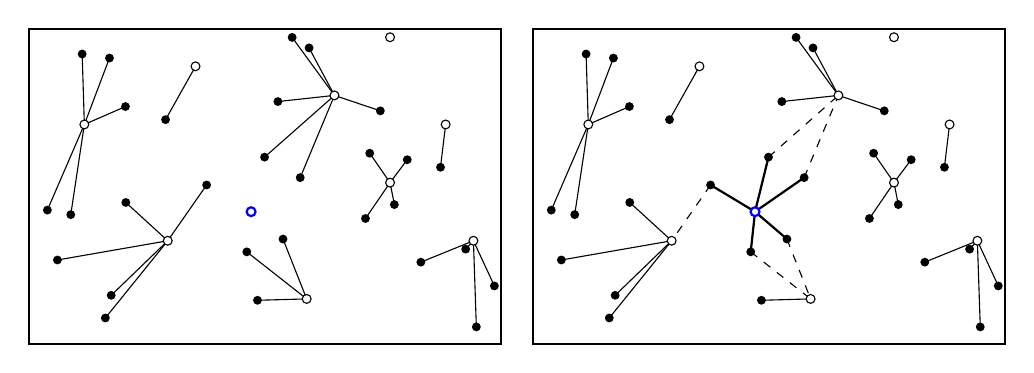
\begin{tikzpicture}[scale=0.4]
\draw [<->,thick] (0,0) rectangle (15,10) {};
\draw [-](7.261764705882353, 1.3796923076923076) -- (8.823529411764707, 1.4230769230769231);
\draw [-](10.690588235294118, 3.9763076923076923) -- (11.470588235294118, 5.115384615384615);
\draw [-](3.0697058823529413, 7.531076923076923) -- (1.7647058823529411, 6.961538461538462);
\draw [-](11.161764705882353, 7.393538461538461) -- (9.705882352941176, 7.884615384615385);
\draw [-](2.4308823529411763, 0.8175384615384615) -- (4.411764705882353, 3.269230769230769);
\draw [-](11.60735294117647, 4.418461538461538) -- (11.470588235294118, 5.115384615384615);
\draw [-](2.617058823529412, 1.5375384615384617) -- (4.411764705882353, 3.269230769230769);
\draw [-](8.617941176470588, 5.274153846153846) -- (9.705882352941176, 7.884615384615385);
\draw [-](0.5902941176470589, 4.243076923076923) -- (1.7647058823529411, 6.961538461538462);
\draw [-](1.695, 9.199076923076923) -- (1.7647058823529411, 6.961538461538462);
\draw [-](4.342941176470588, 7.114769230769231) -- (5.294117647058823, 8.807692307692308);
\draw [-](8.899411764705881, 9.392923076923077) -- (9.705882352941176, 7.884615384615385);
\draw [-](7.485882352941177, 5.924) -- (9.705882352941176, 7.884615384615385);
\draw [-](14.21029411764706, 0.5341538461538462) -- (14.117647058823529, 3.269230769230769);
\draw [-](14.78294117647059, 1.8356923076923077) -- (14.117647058823529, 3.269230769230769);
\draw [-](13.871470588235294, 3.0033846153846158) -- (14.117647058823529, 3.269230769230769);
\draw [-](1.333235294117647, 4.099076923076923) -- (1.7647058823529411, 6.961538461538462);
\draw [-](2.5623529411764707, 9.070769230769232) -- (1.7647058823529411, 6.961538461538462);
\draw [-](12.015882352941176, 5.842769230769231) -- (11.470588235294118, 5.115384615384615);
\draw [-](12.448235294117648, 2.5898461538461537) -- (14.117647058823529, 3.269230769230769);
\draw [-](0.909705882352941, 2.659076923076923) -- (4.411764705882353, 3.269230769230769);
\draw [-](3.0811764705882356, 4.485846153846154) -- (4.411764705882353, 3.269230769230769);
\draw [-](8.362058823529411, 9.726153846153846) -- (9.705882352941176, 7.884615384615385);
\draw [-](10.824705882352943, 6.048615384615385) -- (11.470588235294118, 5.115384615384615);
\draw [-](5.647058823529412, 5.040615384615384) -- (4.411764705882353, 3.269230769230769);
\draw [-](8.071764705882353, 3.3236923076923075) -- (8.823529411764707, 1.4230769230769231);
\draw [-](13.072058823529412, 5.602769230769231) -- (13.235294117647058, 6.961538461538462);
\draw [-](6.922058823529412, 2.917538461538462) -- (8.823529411764707, 1.4230769230769231);
\draw [-](7.909411764705883, 7.688923076923077) -- (9.705882352941176, 7.884615384615385);
\fill [white](1.7647058823529411, 6.961538461538462)circle(4pt);
\draw (1.7647058823529411, 6.961538461538462)circle(4pt);
\fill [white](4.411764705882353, 3.269230769230769)circle(4pt);
\draw (4.411764705882353, 3.269230769230769)circle(4pt);
\fill [white](5.294117647058823, 8.807692307692308)circle(4pt);
\draw (5.294117647058823, 8.807692307692308)circle(4pt);
\fill [white](8.823529411764707, 1.4230769230769231)circle(4pt);
\draw (8.823529411764707, 1.4230769230769231)circle(4pt);
\fill [white](9.705882352941176, 7.884615384615385)circle(4pt);
\draw (9.705882352941176, 7.884615384615385)circle(4pt);
\fill [white](11.470588235294118, 5.115384615384615)circle(4pt);
\draw (11.470588235294118, 5.115384615384615)circle(4pt);
\fill [white](11.470588235294118, 9.73076923076923)circle(4pt);
\draw (11.470588235294118, 9.73076923076923)circle(4pt);
\fill [white](13.235294117647058, 6.961538461538462)circle(4pt);
\draw (13.235294117647058, 6.961538461538462)circle(4pt);
\fill [white](14.117647058823529, 3.269230769230769)circle(4pt);
\draw (14.117647058823529, 3.269230769230769)circle(4pt);
\fill [white](7.0588235294117645, 4.1923076923076925)circle(4pt);
\draw [blue,thick](7.0588235294117645, 4.1923076923076925)circle(4pt);
\fill(7.261764705882353, 1.3796923076923076)circle(4pt);
\fill(10.690588235294118, 3.9763076923076923)circle(4pt);
\fill(3.0697058823529413, 7.531076923076923)circle(4pt);
\fill(11.161764705882353, 7.393538461538461)circle(4pt);
\fill(2.4308823529411763, 0.8175384615384615)circle(4pt);
\fill(11.60735294117647, 4.418461538461538)circle(4pt);
\fill(2.617058823529412, 1.5375384615384617)circle(4pt);
\fill(8.617941176470588, 5.274153846153846)circle(4pt);
\fill(0.5902941176470589, 4.243076923076923)circle(4pt);
\fill(1.695, 9.199076923076923)circle(4pt);
\fill(4.342941176470588, 7.114769230769231)circle(4pt);
\fill(8.899411764705881, 9.392923076923077)circle(4pt);
\fill(7.485882352941177, 5.924)circle(4pt);
\fill(14.21029411764706, 0.5341538461538462)circle(4pt);
\fill(14.78294117647059, 1.8356923076923077)circle(4pt);
\fill(13.871470588235294, 3.0033846153846158)circle(4pt);
\fill(1.333235294117647, 4.099076923076923)circle(4pt);
\fill(2.5623529411764707, 9.070769230769232)circle(4pt);
\fill(12.015882352941176, 5.842769230769231)circle(4pt);
\fill(12.448235294117648, 2.5898461538461537)circle(4pt);
\fill(0.909705882352941, 2.659076923076923)circle(4pt);
\fill(3.0811764705882356, 4.485846153846154)circle(4pt);
\fill(8.362058823529411, 9.726153846153846)circle(4pt);
\fill(10.824705882352943, 6.048615384615385)circle(4pt);
\fill(5.647058823529412, 5.040615384615384)circle(4pt);
\fill(8.071764705882353, 3.3236923076923075)circle(4pt);
\fill(13.072058823529412, 5.602769230769231)circle(4pt);
\fill(6.922058823529412, 2.917538461538462)circle(4pt);
\fill(7.909411764705883, 7.688923076923077)circle(4pt);
\begin{scope}[shift={(16,0)}]
\draw [<->,thick] (0,0) rectangle (15,10) {};
\draw [-](7.261764705882353, 1.3796923076923076) -- (8.823529411764707, 1.4230769230769231);
\draw [-](10.690588235294118, 3.9763076923076923) -- (11.470588235294118, 5.115384615384615);
\draw [-](3.0697058823529413, 7.531076923076923) -- (1.7647058823529411, 6.961538461538462);
\draw [-](11.161764705882353, 7.393538461538461) -- (9.705882352941176, 7.884615384615385);
\draw [-](2.4308823529411763, 0.8175384615384615) -- (4.411764705882353, 3.269230769230769);
\draw [-](11.60735294117647, 4.418461538461538) -- (11.470588235294118, 5.115384615384615);
\draw [-](2.617058823529412, 1.5375384615384617) -- (4.411764705882353, 3.269230769230769);
\draw [-,dashed](8.617941176470588, 5.274153846153846) -- (9.705882352941176, 7.884615384615385);
\draw [-](0.5902941176470589, 4.243076923076923) -- (1.7647058823529411, 6.961538461538462);
\draw [-](1.695, 9.199076923076923) -- (1.7647058823529411, 6.961538461538462);
\draw [-](4.342941176470588, 7.114769230769231) -- (5.294117647058823, 8.807692307692308);
\draw [-](8.899411764705881, 9.392923076923077) -- (9.705882352941176, 7.884615384615385);
\draw [-,dashed](7.485882352941177, 5.924) -- (9.705882352941176, 7.884615384615385);
\draw [-](14.21029411764706, 0.5341538461538462) -- (14.117647058823529, 3.269230769230769);
\draw [-](14.78294117647059, 1.8356923076923077) -- (14.117647058823529, 3.269230769230769);
\draw [-](13.871470588235294, 3.0033846153846158) -- (14.117647058823529, 3.269230769230769);
\draw [-](1.333235294117647, 4.099076923076923) -- (1.7647058823529411, 6.961538461538462);
\draw [-](2.5623529411764707, 9.070769230769232) -- (1.7647058823529411, 6.961538461538462);
\draw [-](12.015882352941176, 5.842769230769231) -- (11.470588235294118, 5.115384615384615);
\draw [-](12.448235294117648, 2.5898461538461537) -- (14.117647058823529, 3.269230769230769);
\draw [-](0.909705882352941, 2.659076923076923) -- (4.411764705882353, 3.269230769230769);
\draw [-](3.0811764705882356, 4.485846153846154) -- (4.411764705882353, 3.269230769230769);
\draw [-](8.362058823529411, 9.726153846153846) -- (9.705882352941176, 7.884615384615385);
\draw [-](10.824705882352943, 6.048615384615385) -- (11.470588235294118, 5.115384615384615);
\draw [-,dashed](5.647058823529412, 5.040615384615384) -- (4.411764705882353, 3.269230769230769);
\draw [-,dashed](8.071764705882353, 3.3236923076923075) -- (8.823529411764707, 1.4230769230769231);
\draw [-](13.072058823529412, 5.602769230769231) -- (13.235294117647058, 6.961538461538462);
\draw [-,dashed](6.922058823529412, 2.917538461538462) -- (8.823529411764707, 1.4230769230769231);
\draw [-](7.909411764705883, 7.688923076923077) -- (9.705882352941176, 7.884615384615385);
\draw [-,thick](8.617941176470588, 5.274153846153846) -- (7.0588235294117645, 4.1923076923076925);
\draw [-,thick](7.485882352941177, 5.924) -- (7.0588235294117645, 4.1923076923076925);
\draw [-,thick](5.647058823529412, 5.040615384615384) -- (7.0588235294117645, 4.1923076923076925);
\draw [-,thick](8.071764705882353, 3.3236923076923075) -- (7.0588235294117645, 4.1923076923076925);
\draw [-,thick](6.922058823529412, 2.917538461538462) -- (7.0588235294117645, 4.1923076923076925);
\fill [white](1.7647058823529411, 6.961538461538462)circle(4pt);
\draw (1.7647058823529411, 6.961538461538462)circle(4pt);
\fill [white](4.411764705882353, 3.269230769230769)circle(4pt);
\draw (4.411764705882353, 3.269230769230769)circle(4pt);
\fill [white](5.294117647058823, 8.807692307692308)circle(4pt);
\draw (5.294117647058823, 8.807692307692308)circle(4pt);
\fill [white](8.823529411764707, 1.4230769230769231)circle(4pt);
\draw (8.823529411764707, 1.4230769230769231)circle(4pt);
\fill [white](9.705882352941176, 7.884615384615385)circle(4pt);
\draw (9.705882352941176, 7.884615384615385)circle(4pt);
\fill [white](11.470588235294118, 5.115384615384615)circle(4pt);
\draw (11.470588235294118, 5.115384615384615)circle(4pt);
\fill [white](11.470588235294118, 9.73076923076923)circle(4pt);
\draw (11.470588235294118, 9.73076923076923)circle(4pt);
\fill [white](13.235294117647058, 6.961538461538462)circle(4pt);
\draw (13.235294117647058, 6.961538461538462)circle(4pt);
\fill [white](14.117647058823529, 3.269230769230769)circle(4pt);
\draw (14.117647058823529, 3.269230769230769)circle(4pt);
\fill [white](7.0588235294117645, 4.1923076923076925)circle(4pt);
\draw [blue,thick](7.0588235294117645, 4.1923076923076925)circle(4pt);
\fill(7.261764705882353, 1.3796923076923076)circle(4pt);
\fill(10.690588235294118, 3.9763076923076923)circle(4pt);
\fill(3.0697058823529413, 7.531076923076923)circle(4pt);
\fill(11.161764705882353, 7.393538461538461)circle(4pt);
\fill(2.4308823529411763, 0.8175384615384615)circle(4pt);
\fill(11.60735294117647, 4.418461538461538)circle(4pt);
\fill(2.617058823529412, 1.5375384615384617)circle(4pt);
\fill(8.617941176470588, 5.274153846153846)circle(4pt);
\fill(0.5902941176470589, 4.243076923076923)circle(4pt);
\fill(1.695, 9.199076923076923)circle(4pt);
\fill(4.342941176470588, 7.114769230769231)circle(4pt);
\fill(8.899411764705881, 9.392923076923077)circle(4pt);
\fill(7.485882352941177, 5.924)circle(4pt);
\fill(14.21029411764706, 0.5341538461538462)circle(4pt);
\fill(14.78294117647059, 1.8356923076923077)circle(4pt);
\fill(13.871470588235294, 3.0033846153846158)circle(4pt);
\fill(1.333235294117647, 4.099076923076923)circle(4pt);
\fill(2.5623529411764707, 9.070769230769232)circle(4pt);
\fill(12.015882352941176, 5.842769230769231)circle(4pt);
\fill(12.448235294117648, 2.5898461538461537)circle(4pt);
\fill(0.909705882352941, 2.659076923076923)circle(4pt);
\fill(3.0811764705882356, 4.485846153846154)circle(4pt);
\fill(8.362058823529411, 9.726153846153846)circle(4pt);
\fill(10.824705882352943, 6.048615384615385)circle(4pt);
\fill(5.647058823529412, 5.040615384615384)circle(4pt);
\fill(8.071764705882353, 3.3236923076923075)circle(4pt);
\fill(13.072058823529412, 5.602769230769231)circle(4pt);
\fill(6.922058823529412, 2.917538461538462)circle(4pt);
\fill(7.909411764705883, 7.688923076923077)circle(4pt);
\end{scope}
\end{tikzpicture}
\caption[Illustration of a centroid insertion.]{Illustration of a centroid insertion. The new point, in blue, changes the assignment of neighbouring points (in dashed lines), to connect to the new closest centroid.}
\label{fig:ncent}
\vspace{-5pt}
\end{figure}

}

\frame{
	\frametitle{Branch-and-bound}
	\begin{itemize}
		\item Inserting a Non-centroid
		\begin{itemize}
			\item Search for closest centroid
			\item Higher coverage value
		\end{itemize}
	\end{itemize}
	\begin{figure}[!h]
\centering
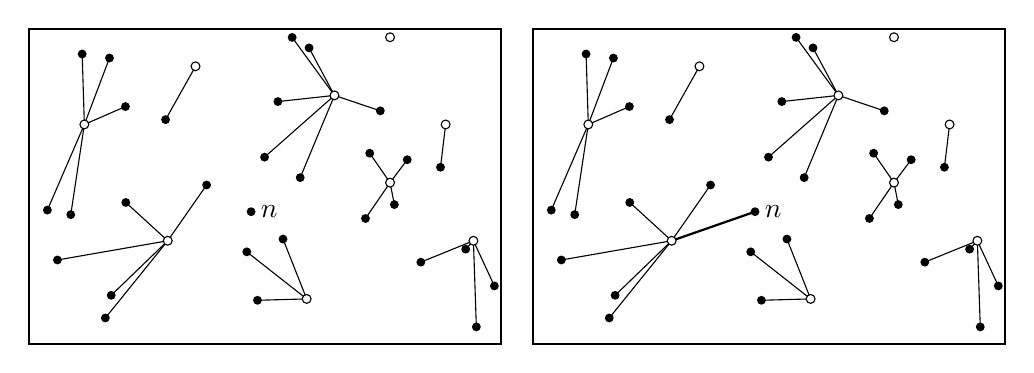
\begin{tikzpicture}[scale=0.4]
\draw [<->,thick] (0,0) rectangle (15,10) {};
\draw [-](7.261764705882353, 1.3796923076923076) -- (8.823529411764707, 1.4230769230769231);
\draw [-](10.690588235294118, 3.9763076923076923) -- (11.470588235294118, 5.115384615384615);
\draw [-](3.0697058823529413, 7.531076923076923) -- (1.7647058823529411, 6.961538461538462);
\draw [-](11.161764705882353, 7.393538461538461) -- (9.705882352941176, 7.884615384615385);
\draw [-](2.4308823529411763, 0.8175384615384615) -- (4.411764705882353, 3.269230769230769);
\draw [-](11.60735294117647, 4.418461538461538) -- (11.470588235294118, 5.115384615384615);
\draw [-](2.617058823529412, 1.5375384615384617) -- (4.411764705882353, 3.269230769230769);
\draw [-](8.617941176470588, 5.274153846153846) -- (9.705882352941176, 7.884615384615385);
\draw [-](0.5902941176470589, 4.243076923076923) -- (1.7647058823529411, 6.961538461538462);
\draw [-](1.695, 9.199076923076923) -- (1.7647058823529411, 6.961538461538462);
\draw [-](4.342941176470588, 7.114769230769231) -- (5.294117647058823, 8.807692307692308);
\draw [-](8.899411764705881, 9.392923076923077) -- (9.705882352941176, 7.884615384615385);
\draw [-](7.485882352941177, 5.924) -- (9.705882352941176, 7.884615384615385);
\draw [-](14.21029411764706, 0.5341538461538462) -- (14.117647058823529, 3.269230769230769);
\draw [-](14.78294117647059, 1.8356923076923077) -- (14.117647058823529, 3.269230769230769);
\draw [-](13.871470588235294, 3.0033846153846158) -- (14.117647058823529, 3.269230769230769);
\draw [-](1.333235294117647, 4.099076923076923) -- (1.7647058823529411, 6.961538461538462);
\draw [-](2.5623529411764707, 9.070769230769232) -- (1.7647058823529411, 6.961538461538462);
\draw [-](12.015882352941176, 5.842769230769231) -- (11.470588235294118, 5.115384615384615);
\draw [-](12.448235294117648, 2.5898461538461537) -- (14.117647058823529, 3.269230769230769);
\draw [-](0.909705882352941, 2.659076923076923) -- (4.411764705882353, 3.269230769230769);
\draw [-](3.0811764705882356, 4.485846153846154) -- (4.411764705882353, 3.269230769230769);
\draw [-](8.362058823529411, 9.726153846153846) -- (9.705882352941176, 7.884615384615385);
\draw [-](10.824705882352943, 6.048615384615385) -- (11.470588235294118, 5.115384615384615);
\draw [-](5.647058823529412, 5.040615384615384) -- (4.411764705882353, 3.269230769230769);
\draw [-](8.071764705882353, 3.3236923076923075) -- (8.823529411764707, 1.4230769230769231);
\draw [-](13.072058823529412, 5.602769230769231) -- (13.235294117647058, 6.961538461538462);
\draw [-](6.922058823529412, 2.917538461538462) -- (8.823529411764707, 1.4230769230769231);
\draw [-](7.909411764705883, 7.688923076923077) -- (9.705882352941176, 7.884615384615385);
\fill [white](1.7647058823529411, 6.961538461538462)circle(4pt);
\draw (1.7647058823529411, 6.961538461538462)circle(4pt);
\fill [white](4.411764705882353, 3.269230769230769)circle(4pt);
\draw (4.411764705882353, 3.269230769230769)circle(4pt);
\fill [white](5.294117647058823, 8.807692307692308)circle(4pt);
\draw (5.294117647058823, 8.807692307692308)circle(4pt);
\fill [white](8.823529411764707, 1.4230769230769231)circle(4pt);
\draw (8.823529411764707, 1.4230769230769231)circle(4pt);
\fill [white](9.705882352941176, 7.884615384615385)circle(4pt);
\draw (9.705882352941176, 7.884615384615385)circle(4pt);
\fill [white](11.470588235294118, 5.115384615384615)circle(4pt);
\draw (11.470588235294118, 5.115384615384615)circle(4pt);
\fill [white](11.470588235294118, 9.73076923076923)circle(4pt);
\draw (11.470588235294118, 9.73076923076923)circle(4pt);
\fill [white](13.235294117647058, 6.961538461538462)circle(4pt);
\draw (13.235294117647058, 6.961538461538462)circle(4pt);
\fill [white](14.117647058823529, 3.269230769230769)circle(4pt);
\draw (14.117647058823529, 3.269230769230769)circle(4pt);
\fill(7.0588235294117645, 4.1923076923076925)circle(4pt);
\fill(7.261764705882353, 1.3796923076923076)circle(4pt);
\fill(10.690588235294118, 3.9763076923076923)circle(4pt);
\fill(3.0697058823529413, 7.531076923076923)circle(4pt);
\fill(11.161764705882353, 7.393538461538461)circle(4pt);
\fill(2.4308823529411763, 0.8175384615384615)circle(4pt);
\fill(11.60735294117647, 4.418461538461538)circle(4pt);
\fill(2.617058823529412, 1.5375384615384617)circle(4pt);
\fill(8.617941176470588, 5.274153846153846)circle(4pt);
\fill(0.5902941176470589, 4.243076923076923)circle(4pt);
\fill(1.695, 9.199076923076923)circle(4pt);
\fill(4.342941176470588, 7.114769230769231)circle(4pt);
\fill(8.899411764705881, 9.392923076923077)circle(4pt);
\fill(7.485882352941177, 5.924)circle(4pt);
\fill(14.21029411764706, 0.5341538461538462)circle(4pt);
\fill(14.78294117647059, 1.8356923076923077)circle(4pt);
\fill(13.871470588235294, 3.0033846153846158)circle(4pt);
\fill(1.333235294117647, 4.099076923076923)circle(4pt);
\fill(2.5623529411764707, 9.070769230769232)circle(4pt);
\fill(12.015882352941176, 5.842769230769231)circle(4pt);
\fill(12.448235294117648, 2.5898461538461537)circle(4pt);
\fill(0.909705882352941, 2.659076923076923)circle(4pt);
\fill(3.0811764705882356, 4.485846153846154)circle(4pt);
\fill(8.362058823529411, 9.726153846153846)circle(4pt);
\fill(10.824705882352943, 6.048615384615385)circle(4pt);
\fill(5.647058823529412, 5.040615384615384)circle(4pt);
\fill(8.071764705882353, 3.3236923076923075)circle(4pt);
\fill(13.072058823529412, 5.602769230769231)circle(4pt);
\fill(6.922058823529412, 2.917538461538462)circle(4pt);
\fill(7.909411764705883, 7.688923076923077)circle(4pt);
\node at (7.0588235294117645, 4.1923076923076925)[right] {$n$};
\begin{scope}[shift={(16,0)}]
\draw [<->,thick] (0,0) rectangle (15,10) {};
\draw [-](7.261764705882353, 1.3796923076923076) -- (8.823529411764707, 1.4230769230769231);
\draw [-](10.690588235294118, 3.9763076923076923) -- (11.470588235294118, 5.115384615384615);
\draw [-](3.0697058823529413, 7.531076923076923) -- (1.7647058823529411, 6.961538461538462);
\draw [-](11.161764705882353, 7.393538461538461) -- (9.705882352941176, 7.884615384615385);
\draw [-](2.4308823529411763, 0.8175384615384615) -- (4.411764705882353, 3.269230769230769);
\draw [-](11.60735294117647, 4.418461538461538) -- (11.470588235294118, 5.115384615384615);
\draw [-](2.617058823529412, 1.5375384615384617) -- (4.411764705882353, 3.269230769230769);
\draw [-](8.617941176470588, 5.274153846153846) -- (9.705882352941176, 7.884615384615385);
\draw [-](0.5902941176470589, 4.243076923076923) -- (1.7647058823529411, 6.961538461538462);
\draw [-](1.695, 9.199076923076923) -- (1.7647058823529411, 6.961538461538462);
\draw [-](4.342941176470588, 7.114769230769231) -- (5.294117647058823, 8.807692307692308);
\draw [-](8.899411764705881, 9.392923076923077) -- (9.705882352941176, 7.884615384615385);
\draw [-](7.485882352941177, 5.924) -- (9.705882352941176, 7.884615384615385);
\draw [-](14.21029411764706, 0.5341538461538462) -- (14.117647058823529, 3.269230769230769);
\draw [-](14.78294117647059, 1.8356923076923077) -- (14.117647058823529, 3.269230769230769);
\draw [-](13.871470588235294, 3.0033846153846158) -- (14.117647058823529, 3.269230769230769);
\draw [-](1.333235294117647, 4.099076923076923) -- (1.7647058823529411, 6.961538461538462);
\draw [-](2.5623529411764707, 9.070769230769232) -- (1.7647058823529411, 6.961538461538462);
\draw [-](12.015882352941176, 5.842769230769231) -- (11.470588235294118, 5.115384615384615);
\draw [-](12.448235294117648, 2.5898461538461537) -- (14.117647058823529, 3.269230769230769);
\draw [-](0.909705882352941, 2.659076923076923) -- (4.411764705882353, 3.269230769230769);
\draw [-](3.0811764705882356, 4.485846153846154) -- (4.411764705882353, 3.269230769230769);
\draw [-](8.362058823529411, 9.726153846153846) -- (9.705882352941176, 7.884615384615385);
\draw [-](10.824705882352943, 6.048615384615385) -- (11.470588235294118, 5.115384615384615);
\draw [-](5.647058823529412, 5.040615384615384) -- (4.411764705882353, 3.269230769230769);
\draw [-](8.071764705882353, 3.3236923076923075) -- (8.823529411764707, 1.4230769230769231);
\draw [-](13.072058823529412, 5.602769230769231) -- (13.235294117647058, 6.961538461538462);
\draw [-](6.922058823529412, 2.917538461538462) -- (8.823529411764707, 1.4230769230769231);
\draw [-](7.909411764705883, 7.688923076923077) -- (9.705882352941176, 7.884615384615385);
\draw [-,thick](7.0588235294117645, 4.1923076923076925) -- (4.411764705882353, 3.269230769230769);
\fill [white](1.7647058823529411, 6.961538461538462)circle(4pt);
\draw (1.7647058823529411, 6.961538461538462)circle(4pt);
\fill [white](4.411764705882353, 3.269230769230769)circle(4pt);
\draw (4.411764705882353, 3.269230769230769)circle(4pt);
\fill [white](5.294117647058823, 8.807692307692308)circle(4pt);
\draw (5.294117647058823, 8.807692307692308)circle(4pt);
\fill [white](8.823529411764707, 1.4230769230769231)circle(4pt);
\draw (8.823529411764707, 1.4230769230769231)circle(4pt);
\fill [white](9.705882352941176, 7.884615384615385)circle(4pt);
\draw (9.705882352941176, 7.884615384615385)circle(4pt);
\fill [white](11.470588235294118, 5.115384615384615)circle(4pt);
\draw (11.470588235294118, 5.115384615384615)circle(4pt);
\fill [white](11.470588235294118, 9.73076923076923)circle(4pt);
\draw (11.470588235294118, 9.73076923076923)circle(4pt);
\fill [white](13.235294117647058, 6.961538461538462)circle(4pt);
\draw (13.235294117647058, 6.961538461538462)circle(4pt);
\fill [white](14.117647058823529, 3.269230769230769)circle(4pt);
\draw (14.117647058823529, 3.269230769230769)circle(4pt);
\fill (7.0588235294117645, 4.1923076923076925)circle(4pt);
\fill(7.261764705882353, 1.3796923076923076)circle(4pt);
\fill(10.690588235294118, 3.9763076923076923)circle(4pt);
\fill(3.0697058823529413, 7.531076923076923)circle(4pt);
\fill(11.161764705882353, 7.393538461538461)circle(4pt);
\fill(2.4308823529411763, 0.8175384615384615)circle(4pt);
\fill(11.60735294117647, 4.418461538461538)circle(4pt);
\fill(2.617058823529412, 1.5375384615384617)circle(4pt);
\fill(8.617941176470588, 5.274153846153846)circle(4pt);
\fill(0.5902941176470589, 4.243076923076923)circle(4pt);
\fill(1.695, 9.199076923076923)circle(4pt);
\fill(4.342941176470588, 7.114769230769231)circle(4pt);
\fill(8.899411764705881, 9.392923076923077)circle(4pt);
\fill(7.485882352941177, 5.924)circle(4pt);
\fill(14.21029411764706, 0.5341538461538462)circle(4pt);
\fill(14.78294117647059, 1.8356923076923077)circle(4pt);
\fill(13.871470588235294, 3.0033846153846158)circle(4pt);
\fill(1.333235294117647, 4.099076923076923)circle(4pt);
\fill(2.5623529411764707, 9.070769230769232)circle(4pt);
\fill(12.015882352941176, 5.842769230769231)circle(4pt);
\fill(12.448235294117648, 2.5898461538461537)circle(4pt);
\fill(0.909705882352941, 2.659076923076923)circle(4pt);
\fill(3.0811764705882356, 4.485846153846154)circle(4pt);
\fill(8.362058823529411, 9.726153846153846)circle(4pt);
\fill(10.824705882352943, 6.048615384615385)circle(4pt);
\fill(5.647058823529412, 5.040615384615384)circle(4pt);
\fill(8.071764705882353, 3.3236923076923075)circle(4pt);
\fill(13.072058823529412, 5.602769230769231)circle(4pt);
\fill(6.922058823529412, 2.917538461538462)circle(4pt);
\fill(7.909411764705883, 7.688923076923077)circle(4pt);
\node at (7.0588235294117645, 4.1923076923076925)[right] {$n$};
\end{scope}
\end{tikzpicture}
\caption[Illustration of a non-centroid insertion]{Illustration of a non-centroid insertion. The new non-centroid, $n$, is assigned to the closest centroid.}
\label{fig:nncent}
\end{figure}

}


\frame{
	\frametitle{Branch-and-bound}
	\begin{itemize}
				\item Removing a Centroid
				\begin{itemize}
					\item Update all non-centroids
					\item Higher coverage value
				\end{itemize}
	\end{itemize}
	\begin{figure}[H]
\centering
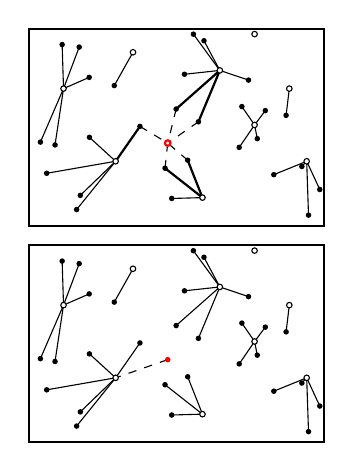
\begin{tikzpicture}[scale=0.25]
\begin{scope}[shift={(0,0)}]\draw [<->,thick] (0,0) rectangle (15,10) {};
\draw [-](7.261764705882353, 1.3796923076923076) -- (8.823529411764707, 1.4230769230769231);
\draw [-](10.690588235294118, 3.9763076923076923) -- (11.470588235294118, 5.115384615384615);
\draw [-](3.0697058823529413, 7.531076923076923) -- (1.7647058823529411, 6.961538461538462);
\draw [-](11.161764705882353, 7.393538461538461) -- (9.705882352941176, 7.884615384615385);
\draw [-](2.4308823529411763, 0.8175384615384615) -- (4.411764705882353, 3.269230769230769);
\draw [-](11.60735294117647, 4.418461538461538) -- (11.470588235294118, 5.115384615384615);
\draw [-](2.617058823529412, 1.5375384615384617) -- (4.411764705882353, 3.269230769230769);
\draw [-,thick](8.617941176470588, 5.274153846153846) -- (9.705882352941176, 7.884615384615385);
\draw [-](0.5902941176470589, 4.243076923076923) -- (1.7647058823529411, 6.961538461538462);
\draw [-](1.695, 9.199076923076923) -- (1.7647058823529411, 6.961538461538462);
\draw [-](4.342941176470588, 7.114769230769231) -- (5.294117647058823, 8.807692307692308);
\draw [-](8.899411764705881, 9.392923076923077) -- (9.705882352941176, 7.884615384615385);
\draw [-,thick](7.485882352941177, 5.924) -- (9.705882352941176, 7.884615384615385);
\draw [-](14.21029411764706, 0.5341538461538462) -- (14.117647058823529, 3.269230769230769);
\draw [-](14.78294117647059, 1.8356923076923077) -- (14.117647058823529, 3.269230769230769);
\draw [-](13.871470588235294, 3.0033846153846158) -- (14.117647058823529, 3.269230769230769);
\draw [-](1.333235294117647, 4.099076923076923) -- (1.7647058823529411, 6.961538461538462);
\draw [-](2.5623529411764707, 9.070769230769232) -- (1.7647058823529411, 6.961538461538462);
\draw [-](12.015882352941176, 5.842769230769231) -- (11.470588235294118, 5.115384615384615);
\draw [-](12.448235294117648, 2.5898461538461537) -- (14.117647058823529, 3.269230769230769);
\draw [-](0.909705882352941, 2.659076923076923) -- (4.411764705882353, 3.269230769230769);
\draw [-](3.0811764705882356, 4.485846153846154) -- (4.411764705882353, 3.269230769230769);
\draw [-](8.362058823529411, 9.726153846153846) -- (9.705882352941176, 7.884615384615385);
\draw [-](10.824705882352943, 6.048615384615385) -- (11.470588235294118, 5.115384615384615);
\draw [-,thick](5.647058823529412, 5.040615384615384) -- (4.411764705882353, 3.269230769230769);
\draw [-,thick](8.071764705882353, 3.3236923076923075) -- (8.823529411764707, 1.4230769230769231);
\draw [-](13.072058823529412, 5.602769230769231) -- (13.235294117647058, 6.961538461538462);
\draw [-,thick](6.922058823529412, 2.917538461538462) -- (8.823529411764707, 1.4230769230769231);
\draw [-](7.909411764705883, 7.688923076923077) -- (9.705882352941176, 7.884615384615385);
\draw [-,dashed](8.617941176470588, 5.274153846153846) -- (7.0588235294117645, 4.1923076923076925);
\draw [-,dashed](7.485882352941177, 5.924) -- (7.0588235294117645, 4.1923076923076925);
\draw [-,dashed](5.647058823529412, 5.040615384615384) -- (7.0588235294117645, 4.1923076923076925);
\draw [-,dashed](8.071764705882353, 3.3236923076923075) -- (7.0588235294117645, 4.1923076923076925);
\draw [-,dashed](6.922058823529412, 2.917538461538462) -- (7.0588235294117645, 4.1923076923076925);
\fill [white](1.7647058823529411, 6.961538461538462)circle(4pt);
\draw (1.7647058823529411, 6.961538461538462)circle(4pt);
\fill [white](4.411764705882353, 3.269230769230769)circle(4pt);
\draw (4.411764705882353, 3.269230769230769)circle(4pt);
\fill [white](5.294117647058823, 8.807692307692308)circle(4pt);
\draw (5.294117647058823, 8.807692307692308)circle(4pt);
\fill [white](8.823529411764707, 1.4230769230769231)circle(4pt);
\draw (8.823529411764707, 1.4230769230769231)circle(4pt);
\fill [white](9.705882352941176, 7.884615384615385)circle(4pt);
\draw (9.705882352941176, 7.884615384615385)circle(4pt);
\fill [white](11.470588235294118, 5.115384615384615)circle(4pt);
\draw (11.470588235294118, 5.115384615384615)circle(4pt);
\fill [white](11.470588235294118, 9.73076923076923)circle(4pt);
\draw (11.470588235294118, 9.73076923076923)circle(4pt);
\fill [white](13.235294117647058, 6.961538461538462)circle(4pt);
\draw (13.235294117647058, 6.961538461538462)circle(4pt);
\fill [white](14.117647058823529, 3.269230769230769)circle(4pt);
\draw (14.117647058823529, 3.269230769230769)circle(4pt);
\fill [white](7.0588235294117645, 4.1923076923076925)circle(4pt);
\draw [red,thick](7.0588235294117645, 4.1923076923076925)circle(4pt);
\fill(7.261764705882353, 1.3796923076923076)circle(4pt);
\fill(10.690588235294118, 3.9763076923076923)circle(4pt);
\fill(3.0697058823529413, 7.531076923076923)circle(4pt);
\fill(11.161764705882353, 7.393538461538461)circle(4pt);
\fill(2.4308823529411763, 0.8175384615384615)circle(4pt);
\fill(11.60735294117647, 4.418461538461538)circle(4pt);
\fill(2.617058823529412, 1.5375384615384617)circle(4pt);
\fill(8.617941176470588, 5.274153846153846)circle(4pt);
\fill(0.5902941176470589, 4.243076923076923)circle(4pt);
\fill(1.695, 9.199076923076923)circle(4pt);
\fill(4.342941176470588, 7.114769230769231)circle(4pt);
\fill(8.899411764705881, 9.392923076923077)circle(4pt);
\fill(7.485882352941177, 5.924)circle(4pt);
\fill(14.21029411764706, 0.5341538461538462)circle(4pt);
\fill(14.78294117647059, 1.8356923076923077)circle(4pt);
\fill(13.871470588235294, 3.0033846153846158)circle(4pt);
\fill(1.333235294117647, 4.099076923076923)circle(4pt);
\fill(2.5623529411764707, 9.070769230769232)circle(4pt);
\fill(12.015882352941176, 5.842769230769231)circle(4pt);
\fill(12.448235294117648, 2.5898461538461537)circle(4pt);
\fill(0.909705882352941, 2.659076923076923)circle(4pt);
\fill(3.0811764705882356, 4.485846153846154)circle(4pt);
\fill(8.362058823529411, 9.726153846153846)circle(4pt);
\fill(10.824705882352943, 6.048615384615385)circle(4pt);
\fill(5.647058823529412, 5.040615384615384)circle(4pt);
\fill(8.071764705882353, 3.3236923076923075)circle(4pt);
\fill(13.072058823529412, 5.602769230769231)circle(4pt);
\fill(6.922058823529412, 2.917538461538462)circle(4pt);
\fill(7.909411764705883, 7.688923076923077)circle(4pt);
\begin{scope}[shift={(0,-11)}]


\draw [<->,thick] (0,0) rectangle (15,10) {};
\draw [-](7.261764705882353, 1.3796923076923076) -- (8.823529411764707, 1.4230769230769231);
\draw [-](10.690588235294118, 3.9763076923076923) -- (11.470588235294118, 5.115384615384615);
\draw [-](3.0697058823529413, 7.531076923076923) -- (1.7647058823529411, 6.961538461538462);
\draw [-](11.161764705882353, 7.393538461538461) -- (9.705882352941176, 7.884615384615385);
\draw [-](2.4308823529411763, 0.8175384615384615) -- (4.411764705882353, 3.269230769230769);
\draw [-](11.60735294117647, 4.418461538461538) -- (11.470588235294118, 5.115384615384615);
\draw [-](2.617058823529412, 1.5375384615384617) -- (4.411764705882353, 3.269230769230769);
\draw [-](8.617941176470588, 5.274153846153846) -- (9.705882352941176, 7.884615384615385);
\draw [-](0.5902941176470589, 4.243076923076923) -- (1.7647058823529411, 6.961538461538462);
\draw [-](1.695, 9.199076923076923) -- (1.7647058823529411, 6.961538461538462);
\draw [-](4.342941176470588, 7.114769230769231) -- (5.294117647058823, 8.807692307692308);
\draw [-](8.899411764705881, 9.392923076923077) -- (9.705882352941176, 7.884615384615385);
\draw [-](7.485882352941177, 5.924) -- (9.705882352941176, 7.884615384615385);
\draw [-](14.21029411764706, 0.5341538461538462) -- (14.117647058823529, 3.269230769230769);
\draw [-](14.78294117647059, 1.8356923076923077) -- (14.117647058823529, 3.269230769230769);
\draw [-](13.871470588235294, 3.0033846153846158) -- (14.117647058823529, 3.269230769230769);
\draw [-](1.333235294117647, 4.099076923076923) -- (1.7647058823529411, 6.961538461538462);
\draw [-](2.5623529411764707, 9.070769230769232) -- (1.7647058823529411, 6.961538461538462);
\draw [-](12.015882352941176, 5.842769230769231) -- (11.470588235294118, 5.115384615384615);
\draw [-](12.448235294117648, 2.5898461538461537) -- (14.117647058823529, 3.269230769230769);
\draw [-](0.909705882352941, 2.659076923076923) -- (4.411764705882353, 3.269230769230769);
\draw [-](3.0811764705882356, 4.485846153846154) -- (4.411764705882353, 3.269230769230769);
\draw [-](8.362058823529411, 9.726153846153846) -- (9.705882352941176, 7.884615384615385);
\draw [-](10.824705882352943, 6.048615384615385) -- (11.470588235294118, 5.115384615384615);
\draw [-](5.647058823529412, 5.040615384615384) -- (4.411764705882353, 3.269230769230769);
\draw [-](8.071764705882353, 3.3236923076923075) -- (8.823529411764707, 1.4230769230769231);
\draw [-](13.072058823529412, 5.602769230769231) -- (13.235294117647058, 6.961538461538462);
\draw [-](6.922058823529412, 2.917538461538462) -- (8.823529411764707, 1.4230769230769231);
\draw [-](7.909411764705883, 7.688923076923077) -- (9.705882352941176, 7.884615384615385);
\draw [-,dashed](7.0588235294117645, 4.1923076923076925) -- (4.411764705882353, 3.269230769230769);
\fill [white](1.7647058823529411, 6.961538461538462)circle(4pt);
\draw (1.7647058823529411, 6.961538461538462)circle(4pt);
\fill [white](4.411764705882353, 3.269230769230769)circle(4pt);
\draw (4.411764705882353, 3.269230769230769)circle(4pt);
\fill [white](5.294117647058823, 8.807692307692308)circle(4pt);
\draw (5.294117647058823, 8.807692307692308)circle(4pt);
\fill [white](8.823529411764707, 1.4230769230769231)circle(4pt);
\draw (8.823529411764707, 1.4230769230769231)circle(4pt);
\fill [white](9.705882352941176, 7.884615384615385)circle(4pt);
\draw (9.705882352941176, 7.884615384615385)circle(4pt);
\fill [white](11.470588235294118, 5.115384615384615)circle(4pt);
\draw (11.470588235294118, 5.115384615384615)circle(4pt);
\fill [white](11.470588235294118, 9.73076923076923)circle(4pt);
\draw (11.470588235294118, 9.73076923076923)circle(4pt);
\fill [white](13.235294117647058, 6.961538461538462)circle(4pt);
\draw (13.235294117647058, 6.961538461538462)circle(4pt);
\fill [white](14.117647058823529, 3.269230769230769)circle(4pt);
\draw (14.117647058823529, 3.269230769230769)circle(4pt);
\fill [red](7.0588235294117645, 4.1923076923076925)circle(4pt);
\fill(7.261764705882353, 1.3796923076923076)circle(4pt);
\fill(10.690588235294118, 3.9763076923076923)circle(4pt);
\fill(3.0697058823529413, 7.531076923076923)circle(4pt);
\fill(11.161764705882353, 7.393538461538461)circle(4pt);
\fill(2.4308823529411763, 0.8175384615384615)circle(4pt);
\fill(11.60735294117647, 4.418461538461538)circle(4pt);
\fill(2.617058823529412, 1.5375384615384617)circle(4pt);
\fill(8.617941176470588, 5.274153846153846)circle(4pt);
\fill(0.5902941176470589, 4.243076923076923)circle(4pt);
\fill(1.695, 9.199076923076923)circle(4pt);
\fill(4.342941176470588, 7.114769230769231)circle(4pt);
\fill(8.899411764705881, 9.392923076923077)circle(4pt);
\fill(7.485882352941177, 5.924)circle(4pt);
\fill(14.21029411764706, 0.5341538461538462)circle(4pt);
\fill(14.78294117647059, 1.8356923076923077)circle(4pt);
\fill(13.871470588235294, 3.0033846153846158)circle(4pt);
\fill(1.333235294117647, 4.099076923076923)circle(4pt);
\fill(2.5623529411764707, 9.070769230769232)circle(4pt);
\fill(12.015882352941176, 5.842769230769231)circle(4pt);
\fill(12.448235294117648, 2.5898461538461537)circle(4pt);
\fill(0.909705882352941, 2.659076923076923)circle(4pt);
\fill(3.0811764705882356, 4.485846153846154)circle(4pt);
\fill(8.362058823529411, 9.726153846153846)circle(4pt);
\fill(10.824705882352943, 6.048615384615385)circle(4pt);
\fill(5.647058823529412, 5.040615384615384)circle(4pt);
\fill(8.071764705882353, 3.3236923076923075)circle(4pt);
\fill(13.072058823529412, 5.602769230769231)circle(4pt);
\fill(6.922058823529412, 2.917538461538462)circle(4pt);
\fill(7.909411764705883, 7.688923076923077)circle(4pt);
\end{scope}
\end{scope}
\end{tikzpicture}
\end{figure}

}


%		\item Removing a Non-centroid
%		\begin{itemize}
%			\item Update objective function
%			\item Smaller coverage value
%		\end{itemize}
%	\end{itemize}
%}

\frame{
	\frametitle{Geometric Approach}	
	\begin{itemize}
		\item Unnecessary number of calculations
		\begin{itemize}	
			\item Use geometric structures to speed objective function update
			\pause
			\item Delaunay triangulations
		\end{itemize}
	\end{itemize}
	\begin{figure}[!h]
	\begin{center}
		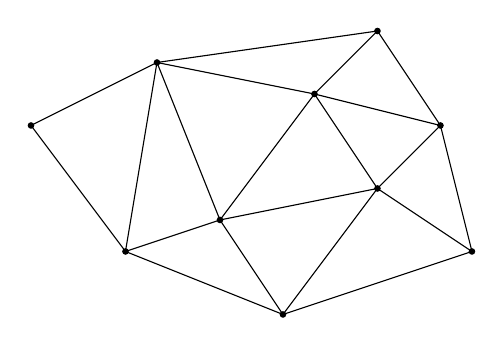
\begin{tikzpicture}[scale=0.4]
		%\draw [<->,thick] (0,10) node (yaxis) [left] {}
		%|- (15,0) node (xaxis) [below] {};
		%centroids
		\fill ( 2, 7) circle (3pt);
		\fill ( 5, 3) circle (3pt);
		\fill ( 6, 9) circle (3pt);
		\fill ( 8, 4) circle (3pt);
		\fill (10, 1) circle (3pt);
		\fill (11, 8) circle (3pt);
		\fill (13, 5) circle (3pt);
		\fill (13,10) circle (3pt);
		\fill (15, 7) circle (3pt);
		\fill (16, 3) circle (3pt);
		
		
		\draw [-] ( 2,7) -- ( 6,9);
		\draw [-] ( 6,9) -- ( 5,3);
		\draw [-] ( 5,3) -- ( 2,7);
		\draw [-] ( 6,9) -- ( 8,4);
		\draw [-] (10,1) -- ( 8,4);
		\draw [-] ( 5,3) -- (10,1);
		\draw [-] ( 8,4) -- ( 5,3);
		\draw [-] ( 8,4) -- (11,8);
		\draw [-] (11,8) -- (6,9);
		\draw [-] ( 6,9) -- (13,10);
		\draw [-] (11,8) -- (13,10);
		\draw [-] (15,7) -- (13,10);
		\draw [-] (16,3) -- (15,7);
		\draw [-] (16,3) -- (10,1);
		\draw [-] (16,3) -- (13,5);
		\draw [-] (13,5) -- (15,7);
		\draw [-] (13,5) -- (10,1);
		\draw [-] (13,5) -- (8,4);
		\draw [-] (13,5) -- (11,8);
		\draw [-] (15,7) -- (11,8);
		\end{tikzpicture}
	\end{center}
	\caption{Example of a Delaunay Triangulation}
	\label{fig:dt1}
\end{figure}
}

\frame{
	\frametitle{Geometric Approach}	
	\begin{itemize}
		\item Greedy Routing
	\end{itemize}
	\begin{figure}[H]
	\begin{center}
		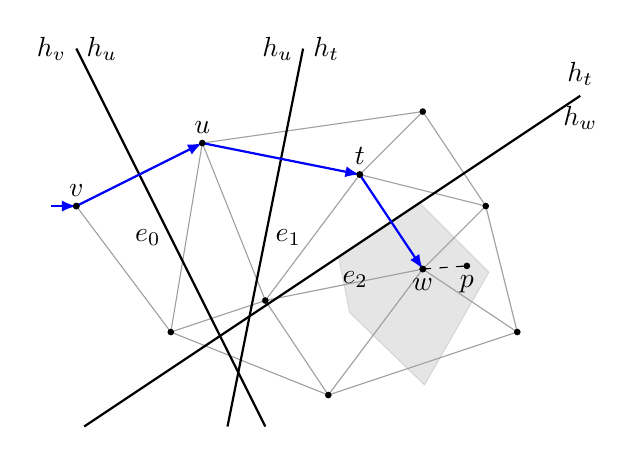
\begin{tikzpicture}[scale=0.4]
		%\draw [<->,thick] (0,10) node (yaxis) [left] {}
		%|- (15,0) node (xaxis) [below] {};
		
		%VORONOI
%		\draw [-,gray!50] ( 5.6764, 5.9706) -- ( 4.9545, 6.0909);
%		\draw [-,gray!50] ( 5.6764, 5.9706) -- ( 8.1956, 6.9783);
%		\draw [-,gray!50] (10.3235, 5.3824) -- ( 8.1956, 6.9783);
%		\draw [-,gray!50] (10.3235, 5.3824) -- (10.6765, 3.6176);
%		\draw [-,gray!50] ( 7.2272, 1.3182) -- (10.6765, 3.6176);
%		\draw [-,gray!50] ( 7.2272, 1.3182) -- ( 5.6764, 5.9706);
%		\draw [-,gray!50] (13.0556, 1.3182) -- (10.6765, 3.6176);
%		\draw [-,gray!50] (13.0556, 1.3182) -- (15.1000, 4.9000);
%		\draw [-,gray!50] (12.9000, 7.1000) -- (15.1000, 4.9000);
%		\draw [-,gray!50] (12.9000, 7.1000) -- (10.3235, 5.3824);
%		\draw [-,gray!50] (12.9000, 7.1000) -- (13.1000, 7.9000);
%		\draw [-,gray!50] ( 9.1667,11.8333) -- (13.1000, 7.9000);
%		%\draw [-,gray!50] ( 9.1667,11.8333) -- ( 8.1956, 6.9783);
%		%VORONOI EXTENDED
%		\draw [-,gray!50] ( 4.9545, 6.0909) -- (2 , 12);
%		\draw [-,gray!50] ( 4.9545, 6.0909) -- (0, 2.375);
%		\draw [-,gray!50] ( 7.2272, 1.3182) -- ( 6.7, 0);
%		\draw [-,gray!50] (13.0556, 1.3182) -- (13.6667, 0);
%		\draw [-,gray!50] (15.1000, 4.9000) -- (18, 5.625);
%		\draw [-,gray!50] (13.1000, 7.9000) -- (18, 11.1667);
%		\draw [-,gray!50] ( 9.1667,11.8333) -- ( 9.1429, 12);
		
		\filldraw[fill=black, opacity=0.1] 	(10.3235, 5.3824) -- (10.6765, 3.6176) --
											(13.0556, 1.3182) -- (15.1000, 4.9000) --
											(12.9000, 7.1000) -- cycle;
		
		%DELAUNAY
		\draw [-,gray!75] ( 2,7) -- ( 6,9);
		\draw [-,gray!75] ( 6,9) -- ( 5,3);
		\draw [-,gray!75] ( 5,3) -- ( 2,7);
		\draw [-,gray!75] ( 6,9) -- ( 8,4);
		\draw [-,gray!75] (10,1) -- ( 8,4);
		\draw [-,gray!75] ( 5,3) -- (10,1);
		\draw [-,gray!75] ( 8,4) -- ( 5,3);
		\draw [-,gray!75] ( 8,4) -- (11,8);
		\draw [-,gray!75] (11,8) -- (6,9);
		\draw [-,gray!75] ( 6,9) -- (13,10);
		\draw [-,gray!75] (11,8) -- (13,10);
		\draw [-,gray!75] (15,7) -- (13,10);
		\draw [-,gray!75] (16,3) -- (15,7);
		\draw [-,gray!75] (16,3) -- (10,1);
		\draw [-,gray!75] (16,3) -- (13,5);
		\draw [-,gray!75] (13,5) -- (15,7);
		\draw [-,gray!75] (13,5) -- (10,1);
		\draw [-,gray!75] (13,5) -- (8,4);
		\draw [-,gray!75] (13,5) -- (11,8);
		\draw [-,gray!75] (15,7) -- (11,8);
		
		
		%POINTS
		
		\fill ( 2, 7) circle (3pt);
		\fill ( 5, 3) circle (3pt);
		\fill ( 8, 4) circle (3pt);
		\fill (10, 1) circle (3pt);
		\fill (11, 8) circle (3pt);
		\fill (13, 5) circle (3pt);
		\fill (13,10) circle (3pt);
		\fill (15, 7) circle (3pt);
		\fill (16, 3) circle (3pt);
		
		%EDGE E
		\draw [-,thick] ( 8,0)		-- node[left]{$e_0$} ( 2, 12)	node[left]		{$h_v$} node[right]{$h_u$};
		\draw [-,thick] ( 6.8,0)	-- node[right]{$e_1$} (9.2,12)	node[left] 		{$h_u$} node[right]{$h_t$};
		\draw [-,thick] ( 2.25,0)	-- node[below right]{$e_2$} (18,10.5)	node[above]{$h_t$} node[below]{$h_w$};
		
		
		\draw [-,dashed]( 13,5) -- ( 14.4, 5.1);
		\draw [->,>=latex,thick,blue]( 1.2,7) -- (  2,7);
		\draw [->,>=latex,thick,blue]( 2,7) -- (  6,9);
		\draw [->,>=latex,thick,blue]( 6,9) -- ( 11, 8);
		\draw [->,>=latex,thick,blue](11,8) -- ( 13, 5);
		\fill (14.4, 5.1) circle (3pt) node[anchor=north]{$p$};
		\fill ( 2, 7)     circle (3pt) node[anchor=south]{$v$};
		\fill ( 6, 9)     circle (3pt) node[anchor=south]{$u$};
		\fill (11, 8)     circle (3pt) node[anchor=south]{$t$};
		\fill (13, 5)     circle (3pt) node[anchor=north]{$w$};
		
		\end{tikzpicture}
	\end{center}
\end{figure}
}

\frame{
	\frametitle{Geometric Approach}	
	\begin{itemize}
		\item Greedy Routing
		\item Use Hilbert curves to minimise distance between consecutive routing calls
	\end{itemize}
	\begin{figure}[H]
	\begin{center}
		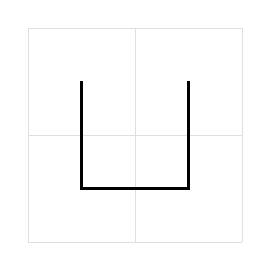
\begin{tikzpicture}[scale=0.17]
		\draw [step=8,gray,very thin,opacity=0.25](0,0) grid(16,16);
		\draw [-,thick] 	(4,12) -- ( 4,4) -- ( 12,4) -- ( 12,12);
		\end{tikzpicture}
		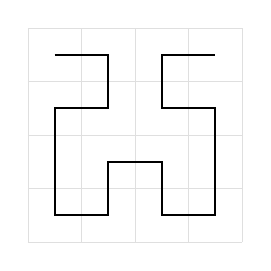
\begin{tikzpicture}[scale=0.17]
		\draw [step=4,gray,very thin,opacity=0.25](0,0) grid(16,16);
		\draw [-,thick]
				 	(2,14) -- ( 6,14) -- (6,10) -- (2,10) -- 
					(2,2)  -- (6,2) -- (6,6) -- (10,6) -- 
					(10,2) -- (14,2) -- (14,10)--(10,10) --
					(10,14) -- (14,14);
		\end{tikzpicture}
		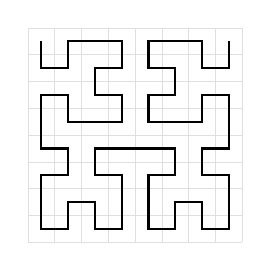
\begin{tikzpicture}[scale=0.17]
		\draw [step=2,gray,very thin,opacity=0.25](0,0) grid(16,16);
		\draw [-,thick] 
					(1,15) 	-- (1,13) 	-- (3,13) 	-- (3,15) 	-- (7,15) 	--
					(7,13) 	-- (5,13) 	-- (5,11)	-- (7,11) 	-- (7,9) 	--
					(3,9) 	-- (3,11)	-- (1,11)	-- (1,7) 	-- (3,7) 	--
					(3,5) 	-- (1,5) 	-- (1,1)	-- (3,1) 	-- (3,3) 	-- 
					(5,3) 	-- (5,1) 	-- (7,1)  	-- (7,5) 	-- (5,5) 	--
					(5,7) 	-- (11,7) 	-- (11,5)  	-- (9,5) 	-- (9,1) 	--
					(11,1)	-- (11,3) 	-- (13,3)  	-- (13,1) 	-- (15,1) 	--
					(15,5) 	-- (13,5) 	-- (13,7)  	-- (15,7) 	-- (15,11)	--
					(13,11)	-- (13,9)  	-- (9,9) 	-- (9,11) 	-- (11,11)	--
					(11,13)	-- (9,13) 	-- (9,15) 	-- (13,15)  -- (13,13) 	--
					(15,13) -- (15,15)
					;
		
		\end{tikzpicture}
		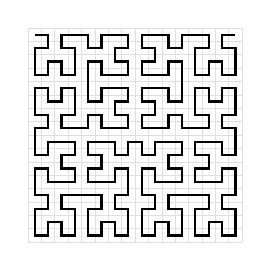
\begin{tikzpicture}[scale=0.17]
		\draw [step=1,gray,very thin,opacity=0.25](0,0) grid(16,16);
		\draw [-,thick] 
				(0.5, 15.5)	-- (1.5, 15.5) 	-- (1.5, 14.5) 	-- (0.5, 14.5) 	-- 
				(0.5, 13.5)	-- (0.5, 12.5) 	-- (1.5, 12.5) 	-- (1.5, 13.5) 	-- 
				(2.5, 13.5)	-- (2.5, 12.5) 	-- (3.5, 12.5) 	-- (3.5, 13.5) 	-- 
				(3.5, 14.5) -- (2.5, 14.5) 	-- (2.5, 15.5) 	-- (3.5, 15.5) 	-- 
				(4.5, 15.5) -- (4.5, 14.5) 	-- (5.5, 14.5) 	-- (5.5, 15.5) 	-- 
				(6.5, 15.5) -- (7.5, 15.5) 	-- (7.5, 14.5) 	-- (6.5, 14.5) 	-- 
				(6.5, 13.5) -- (7.5, 13.5) 	-- (7.5, 12.5) 	-- (6.5, 12.5) 	-- 
				(5.5, 12.5) -- (5.5, 13.5) 	-- (4.5, 13.5) 	-- (4.5, 12.5) 	-- 
				(4.5, 11.5) -- (4.5, 10.5) 	-- (5.5, 10.5) 	-- (5.5, 11.5) 	-- 
				(6.5, 11.5) -- (7.5, 11.5) 	-- (7.5, 10.5) 	-- (6.5, 10.5) 	-- 
				(6.5, 9.5) 	-- (7.5, 9.5) 	-- (7.5, 8.5) 	-- (6.5, 8.5) 	-- 
				(5.5, 8.5) 	-- (5.5, 9.5) 	-- (4.5, 9.5) 	-- (4.5, 8.5) 	-- 
				(3.5, 8.5) 	-- (2.5, 8.5) 	-- (2.5, 9.5) 	-- (3.5, 9.5) 	-- 
				(3.5, 10.5) -- (3.5, 11.5) 	-- (2.5, 11.5) 	-- (2.5, 10.5) 	-- 
				(1.5, 10.5) -- (1.5, 11.5) 	-- (0.5, 11.5) 	-- (0.5, 10.5) 	-- 
				(0.5, 9.5) 	-- (1.5, 9.5)	-- (1.5, 8.5) 	-- (0.5, 8.5) 	-- 
				(0.5, 7.5) 	-- (0.5, 6.5) 	-- (1.5, 6.5) 	-- (1.5, 7.5) 	-- 
				(2.5, 7.5) 	-- (3.5, 7.5) 	-- (3.5, 6.5) 	-- (2.5, 6.5) 	-- 
				(2.5, 5.5) 	-- (3.5, 5.5) 	-- (3.5, 4.5) 	-- (2.5, 4.5) 	-- 
				(1.5, 4.5) 	-- (1.5, 5.5) 	-- (0.5, 5.5) 	-- (0.5, 4.5) 	-- 
				(0.5, 3.5) 	-- (1.5, 3.5) 	-- (1.5, 2.5) 	-- (0.5, 2.5) 	-- 
				(0.5, 1.5) 	-- (0.5, 0.5) 	-- (1.5, 0.5)	-- (1.5, 1.5) 	-- 
				(2.5, 1.5) 	-- (2.5, 0.5) 	-- (3.5, 0.5) 	-- (3.5, 1.5) 	-- 
				(3.5, 2.5) 	-- (2.5, 2.5) 	-- (2.5, 3.5) 	-- (3.5, 3.5) 	-- 
				(4.5, 3.5) 	-- (5.5, 3.5) 	-- (5.5, 2.5) 	-- (4.5, 2.5) 	-- 
				(4.5, 1.5) 	-- (4.5, 0.5) 	-- (5.5, 0.5) 	-- (5.5, 1.5) 	-- 
				(6.5, 1.5) 	-- (6.5, 0.5) 	-- (7.5, 0.5) 	-- (7.5, 1.5) 	-- 
				(7.5, 2.5) 	-- (6.5, 2.5) 	-- (6.5, 3.5) 	-- (7.5, 3.5) 	-- 
				(7.5, 4.5) 	-- (7.5, 5.5) 	-- (6.5, 5.5) 	-- (6.5, 4.5) 	-- 
				(5.5, 4.5) 	-- (4.5, 4.5) 	-- (4.5, 5.5) 	-- (5.5, 5.5) 	-- 
				(5.5, 6.5) 	-- (4.5, 6.5) 	-- (4.5, 7.5) 	-- (5.5, 7.5) 	-- 
				(6.5, 7.5) 	-- (6.5, 6.5) 	-- (7.5, 6.5) 	-- (7.5, 7.5) 	-- 
				(8.5, 7.5) 	-- (8.5, 6.5) 	-- (9.5, 6.5) 	-- (9.5, 7.5) 	-- 
				(10.5, 7.5) -- (11.5, 7.5) 	-- (11.5, 6.5) 	-- (10.5, 6.5) 	-- 
				(10.5, 5.5)	-- (11.5, 5.5) 	-- (11.5, 4.5) 	-- (10.5, 4.5) 	-- 
				(9.5, 4.5) 	-- (9.5, 5.5) 	-- (8.5, 5.5) 	-- (8.5, 4.5) 	-- 
				(8.5, 3.5) 	-- (9.5, 3.5) 	-- (9.5, 2.5) 	-- (8.5, 2.5) 	-- 
				(8.5, 1.5) 	-- (8.5, 0.5) 	-- (9.5, 0.5) 	-- (9.5, 1.5) 	-- 
				(10.5, 1.5) -- (10.5, 0.5) 	-- (11.5, 0.5) 	-- (11.5, 1.5) 	-- 
				(11.5, 2.5) -- (10.5, 2.5) 	-- (10.5, 3.5) 	-- (11.5, 3.5) 	-- 
				(12.5, 3.5) -- (13.5, 3.5)	-- (13.5, 2.5) 	-- (12.5, 2.5) 	-- 
				(12.5, 1.5) -- (12.5, 0.5) 	-- (13.5, 0.5) 	-- (13.5, 1.5) 	-- 
				(14.5, 1.5) -- (14.5, 0.5) 	-- (15.5, 0.5) 	-- (15.5, 1.5) 	-- 
				(15.5, 2.5) -- (14.5, 2.5) 	-- (14.5, 3.5) 	-- (15.5, 3.5) 	-- 
				(15.5, 4.5) -- (15.5, 5.5) 	-- (14.5, 5.5) 	-- (14.5, 4.5) 	-- 
				(13.5, 4.5) -- (12.5, 4.5) 	-- (12.5, 5.5) 	-- (13.5, 5.5) 	-- 
				(13.5, 6.5) -- (12.5, 6.5) 	-- (12.5, 7.5) 	-- (13.5, 7.5) 	-- 
				(14.5, 7.5) -- (14.5, 6.5) 	-- (15.5, 6.5) 	-- (15.5, 7.5) 	-- 
				(15.5, 8.5) -- (14.5, 8.5) 	-- (14.5, 9.5) 	-- (15.5, 9.5) 	-- 
				(15.5, 10.5)-- (15.5, 11.5)	-- (14.5, 11.5)	-- (14.5, 10.5)	-- 
				(13.5, 10.5)-- (13.5, 11.5)	-- (12.5, 11.5)	-- (12.5, 10.5)	--
				(12.5, 9.5)	-- (13.5, 9.5) 	-- (13.5, 8.5)	-- (12.5, 8.5) 	-- 
				(11.5, 8.5) -- (11.5, 9.5) 	-- (10.5, 9.5) 	-- (10.5, 8.5) 	-- 
				(9.5, 8.5) 	-- (8.5, 8.5) 	-- (8.5, 9.5) 	-- (9.5, 9.5) 	--
				(9.5, 10.5) -- (8.5, 10.5) 	-- (8.5, 11.5) 	-- (9.5, 11.5) 	-- 
				(10.5, 11.5)-- (10.5, 10.5)	-- (11.5, 10.5)	-- (11.5, 11.5)	-- 
				(11.5, 12.5)-- (11.5, 13.5)	-- (10.5, 13.5)	-- (10.5, 12.5)	-- 
				(9.5, 12.5) -- (8.5, 12.5) 	-- (8.5, 13.5) 	-- (9.5, 13.5) 	-- 
				(9.5, 14.5) -- (8.5, 14.5) 	-- (8.5, 15.5) 	-- (9.5, 15.5) 	--
				(10.5, 15.5)-- (10.5, 14.5)	-- (11.5, 14.5)	-- (11.5, 15.5)	-- 
				(12.5, 15.5)-- (13.5, 15.5)	-- (13.5, 14.5)	-- (12.5, 14.5)	-- 
				(12.5, 13.5)-- (12.5, 12.5)	-- (13.5, 12.5)	-- (13.5, 13.5)	--
				(14.5, 13.5)-- (14.5, 12.5)	-- (15.5, 12.5)	-- (15.5, 13.5)	--
				(15.5, 14.5)-- (14.5, 14.5)	-- (14.5, 15.5)	-- (15.5, 15.5)
		;		
		\end{tikzpicture}
		
\begin{tikzpicture}[scale=0.17]
		\draw [step=0.5,gray,very thin,opacity=0.25](0,0) grid(16,16);
		\draw [-,thick]
					(15.75,15.75)	--(15.75, 15.25) 	-- (15.25, 15.25) 	-- (15.25, 15.75) 	-- (14.75, 15.75) 	-- (14.25, 15.75) 	-- (14.25, 15.25) 	-- (14.75, 15.25) 	-- (14.75, 14.75) 	-- (14.25, 14.75) 	-- (14.25, 14.25) 	-- (14.75, 14.25) 	-- (15.25, 14.25) 	-- (15.25, 14.75) 	-- (15.75, 14.75) 	-- (15.75, 14.25) 	-- (15.75, 13.75) 	-- (15.25, 13.75) 	-- (15.25, 13.25) 	-- (15.75, 13.25) 	-- (15.75, 12.75) 	-- (15.75, 12.25) 	-- (15.25, 12.25) 	-- (15.25, 12.75) 	-- (14.75, 12.75) 	-- (14.75, 12.25) 	-- (14.25, 12.25) 	-- (14.25, 12.75) 	-- (14.25, 13.25) 	-- (14.75, 13.25) 	-- (14.75, 13.75) 	-- (14.25, 13.75) 	-- (13.75, 13.75) 	-- (13.25, 13.75) 	-- (13.25, 13.25) 	-- (13.75, 13.25) 	-- (13.75, 12.75) 	-- (13.75, 12.25) 	-- (13.25, 12.25) 	-- (13.25, 12.75) 	-- (12.75, 12.75) 	-- (12.75, 12.25) 	-- (12.25, 12.25) 	-- (12.25, 12.75) 	-- (12.25, 13.25) 	-- (12.75, 13.25) 	-- (12.75, 13.75) 	-- (12.25, 13.75) 	-- (12.25, 14.25) 	-- (12.25, 14.75) 	-- (12.75, 14.75) 	-- (12.75, 14.25) 	-- (13.25, 14.25) 	-- (13.75, 14.25) 	-- (13.75, 14.75) 	-- (13.25, 14.75) 	-- (13.25, 15.25) 	-- (13.75, 15.25) 	-- (13.75, 15.75) 	-- (13.25, 15.75) 	-- (12.75, 15.75) 	-- (12.75, 15.25) 	-- (12.25, 15.25) 	-- (12.25, 15.75) 	-- (11.75, 15.75) 	-- (11.25, 15.75) 	-- (11.25, 15.25) 	-- (11.75, 15.25) 	-- (11.75, 14.75) 	-- (11.75, 14.25) 	-- (11.25, 14.25) 	-- (11.25, 14.75) 	-- (10.75, 14.75) 	-- (10.75, 14.25) 	-- (10.25, 14.25) 	-- (10.25, 14.75) 	-- (10.25, 15.25) 	-- (10.75, 15.25) 	-- (10.75, 15.75) 	-- (10.25, 15.75) 	-- (9.75, 15.75) 	-- (9.75, 15.25) 	-- (9.25, 15.25) 	-- (9.25, 15.75) 	-- (8.75, 15.75) 	-- (8.25, 15.75) 	-- (8.25, 15.25) 	-- (8.75, 15.25) 	-- (8.75, 14.75) 	-- (8.25, 14.75) 	-- (8.25, 14.25) 	-- (8.75, 14.25) 	-- (9.25, 14.25) 	-- (9.25, 14.75) 	-- (9.75, 14.75) 	-- (9.75, 14.25) 	-- (9.75, 13.75) 	-- (9.75, 13.25) 	-- (9.25, 13.25) 	-- (9.25, 13.75) 	-- (8.75, 13.75) 	-- (8.25, 13.75) 	-- (8.25, 13.25) 	-- (8.75, 13.25) 	-- (8.75, 12.75) 	-- (8.25, 12.75) 	-- (8.25, 12.25) 	-- (8.75, 12.25) 	-- (9.25, 12.25) 	-- (9.25, 12.75) 	-- (9.75, 12.75) 	-- (9.75, 12.25) 	-- (10.25, 12.25) 	-- (10.75, 12.25) 	-- (10.75, 12.75) 	-- (10.25, 12.75) 	-- (10.25, 13.25) 	-- (10.25, 13.75) 	-- (10.75, 13.75) 	-- (10.75, 13.25) 	-- (11.25, 13.25) 	-- (11.25, 13.75) 	-- (11.75, 13.75) 	-- (11.75, 13.25) 	-- (11.75, 12.75) 	-- (11.25, 12.75) 	-- (11.25, 12.25) 	-- (11.75, 12.25) 	-- (11.75, 11.75) 	-- (11.25, 11.75) 	-- (11.25, 11.25) 	-- (11.75, 11.25) 	-- (11.75, 10.75) 	-- (11.75, 10.25) 	-- (11.25, 10.25) 	-- (11.25, 10.75) 	-- (10.75, 10.75) 	-- (10.75, 10.25) 	-- (10.25, 10.25) 	-- (10.25, 10.75) 	-- (10.25, 11.25) 	-- (10.75, 11.25) 	-- (10.75, 11.75) 	-- (10.25, 11.75) 	-- (9.75, 11.75) 	-- (9.75, 11.25) 	-- (9.25, 11.25) 	-- (9.25, 11.75) 	-- (8.75, 11.75) 	-- (8.25, 11.75) 	-- (8.25, 11.25) 	-- (8.75, 11.25) 	-- (8.75, 10.75) 	-- (8.25, 10.75) 	-- (8.25, 10.25) 	-- (8.75, 10.25) 	-- (9.25, 10.25) 	-- (9.25, 10.75) 	-- (9.75, 10.75) 	-- (9.75, 10.25) 	-- (9.75, 9.75) 	-- (9.75, 9.25) 	-- (9.25, 9.25) 	-- (9.25, 9.75) 	-- (8.75, 9.75) 	-- (8.25, 9.75) 	-- (8.25, 9.25) 	-- (8.75, 9.25) 	-- (8.75, 8.75) 	-- (8.25, 8.75) 	-- (8.25, 8.25) 	-- (8.75, 8.25) 	-- (9.25, 8.25) 	-- (9.25, 8.75) 	-- (9.75, 8.75) 	-- (9.75, 8.25) 	-- (10.25, 8.25) 	-- (10.75, 8.25) 	-- (10.75, 8.75) 	-- (10.25, 8.75) 	-- (10.25, 9.25) 	-- (10.25, 9.75) 	-- (10.75, 9.75) 	-- (10.75, 9.25) 	-- (11.25, 9.25) 	-- (11.25, 9.75) 	-- (11.75, 9.75) 	-- (11.75, 9.25) 	-- (11.75, 8.75) 	-- (11.25, 8.75) 	-- (11.25, 8.25) 	-- (11.75, 8.25) 	-- (12.25, 8.25) 	-- (12.25, 8.75) 	-- (12.75, 8.75) 	-- (12.75, 8.25) 	-- (13.25, 8.25) 	-- (13.75, 8.25) 	-- (13.75, 8.75) 	-- (13.25, 8.75) 	-- (13.25, 9.25) 	-- (13.75, 9.25) 	-- (13.75, 9.75) 	-- (13.25, 9.75) 	-- (12.75, 9.75) 	-- (12.75, 9.25) 	-- (12.25, 9.25) 	-- (12.25, 9.75) 	-- (12.25, 10.25) 	-- (12.75, 10.25) 	-- (12.75, 10.75) 	-- (12.25, 10.75) 	-- (12.25, 11.25) 	-- (12.25, 11.75) 	-- (12.75, 11.75) 	-- (12.75, 11.25) 	-- (13.25, 11.25) 	-- (13.25, 11.75) 	-- (13.75, 11.75) 	-- (13.75, 11.25) 	-- (13.75, 10.75) 	-- (13.25, 10.75) 	-- (13.25, 10.25) 	-- (13.75, 10.25) 	-- (14.25, 10.25) 	-- (14.75, 10.25) 	-- (14.75, 10.75) 	-- (14.25, 10.75) 	-- (14.25, 11.25) 	-- (14.25, 11.75) 	-- (14.75, 11.75) 	-- (14.75, 11.25) 	-- (15.25, 11.25) 	-- (15.25, 11.75) 	-- (15.75, 11.75) 	-- (15.75, 11.25) 	-- (15.75, 10.75) 	-- (15.25, 10.75) 	-- (15.25, 10.25) 	-- (15.75, 10.25) 	-- (15.75, 9.75) 	-- (15.75, 9.25) 	-- (15.25, 9.25) 	-- (15.25, 9.75) 	-- (14.75, 9.75) 	-- (14.25, 9.75) 	-- (14.25, 9.25) 	-- (14.75, 9.25) 	-- (14.75, 8.75) 	-- (14.25, 8.75) 	-- (14.25, 8.25) 	-- (14.75, 8.25) 	-- (15.25, 8.25) 	-- (15.25, 8.75) 	-- (15.75, 8.75) 	-- (15.75, 8.25) 	-- (15.75, 7.75) 	-- (15.25, 7.75) 	-- (15.25, 7.25) 	-- (15.75, 7.25) 	-- (15.75, 6.75) 	-- (15.75, 6.25) 	-- (15.25, 6.25) 	-- (15.25, 6.75) 	-- (14.75, 6.75) 	-- (14.75, 6.25) 	-- (14.25, 6.25) 	-- (14.25, 6.75) 	-- (14.25, 7.25) 	-- (14.75, 7.25) 	-- (14.75, 7.75) 	-- (14.25, 7.75) 	-- (13.75, 7.75) 	-- (13.75, 7.25) 	-- (13.25, 7.25) 	-- (13.25, 7.75) 	-- (12.75, 7.75) 	-- (12.25, 7.75) 	-- (12.25, 7.25) 	-- (12.75, 7.25) 	-- (12.75, 6.75) 	-- (12.25, 6.75) 	-- (12.25, 6.25) 	-- (12.75, 6.25) 	-- (13.25, 6.25) 	-- (13.25, 6.75) 	-- (13.75, 6.75) 	-- (13.75, 6.25) 	-- (13.75, 5.75) 	-- (13.75, 5.25) 	-- (13.25, 5.25) 	-- (13.25, 5.75) 	-- (12.75, 5.75) 	-- (12.25, 5.75) 	-- (12.25, 5.25) 	-- (12.75, 5.25) 	-- (12.75, 4.75) 	-- (12.25, 4.75) 	-- (12.25, 4.25) 	-- (12.75, 4.25) 	-- (13.25, 4.25) 	-- (13.25, 4.75) 	-- (13.75, 4.75) 	-- (13.75, 4.25) 	-- (14.25, 4.25) 	-- (14.75, 4.25) 	-- (14.75, 4.75) 	-- (14.25, 4.75) 	-- (14.25, 5.25) 	-- (14.25, 5.75) 	-- (14.75, 5.75) 	-- (14.75, 5.25) 	-- (15.25, 5.25) 	-- (15.25, 5.75) 	-- (15.75, 5.75) 	-- (15.75, 5.25) 	-- (15.75, 4.75) 	-- (15.25, 4.75) 	-- (15.25, 4.25) 	-- (15.75, 4.25) 	-- (15.75, 3.75) 	-- (15.75, 3.25) 	-- (15.25, 3.25) 	-- (15.25, 3.75) 	-- (14.75, 3.75) 	-- (14.25, 3.75) 	-- (14.25, 3.25) 	-- (14.75, 3.25) 	-- (14.75, 2.75) 	-- (14.25, 2.75) 	-- (14.25, 2.25) 	-- (14.75, 2.25) 	-- (15.25, 2.25) 	-- (15.25, 2.75) 	-- (15.75, 2.75) 	-- (15.75, 2.25) 	-- (15.75, 1.75) 	-- (15.25, 1.75) 	-- (15.25, 1.25) 	-- (15.75, 1.25) 	-- (15.75, 0.75) 	-- (15.75, 0.25) 	-- (15.25, 0.25) 	-- (15.25, 0.75) 	-- (14.75, 0.75) 	-- (14.75, 0.25) 	-- (14.25, 0.25) 	-- (14.25, 0.75) 	-- (14.25, 1.25) 	-- (14.75, 1.25) 	-- (14.75, 1.75) 	-- (14.25, 1.75) 	-- (13.75, 1.75) 	-- (13.25, 1.75) 	-- (13.25, 1.25) 	-- (13.75, 1.25) 	-- (13.75, 0.75) 	-- (13.75, 0.25) 	-- (13.25, 0.25) 	-- (13.25, 0.75) 	-- (12.75, 0.75) 	-- (12.75, 0.25) 	-- (12.25, 0.25) 	-- (12.25, 0.75) 	-- (12.25, 1.25) 	-- (12.75, 1.25) 	-- (12.75, 1.75) 	-- (12.25, 1.75) 	-- (12.25, 2.25) 	-- (12.25, 2.75) 	-- (12.75, 2.75) 	-- (12.75, 2.25) 	-- (13.25, 2.25) 	-- (13.75, 2.25) 	-- (13.75, 2.75) 	-- (13.25, 2.75) 	-- (13.25, 3.25) 	-- (13.75, 3.25) 	-- (13.75, 3.75) 	-- (13.25, 3.75) 	-- (12.75, 3.75) 	-- (12.75, 3.25) 	-- (12.25, 3.25) 	-- (12.25, 3.75) 	-- (11.75, 3.75) 	-- (11.75, 3.25) 	-- (11.25, 3.25) 	-- (11.25, 3.75) 	-- (10.75, 3.75) 	-- (10.25, 3.75) 	-- (10.25, 3.25) 	-- (10.75, 3.25) 	-- (10.75, 2.75) 	-- (10.25, 2.75) 	-- (10.25, 2.25) 	-- (10.75, 2.25) 	-- (11.25, 2.25) 	-- (11.25, 2.75) 	-- (11.75, 2.75) 	-- (11.75, 2.25) 	-- (11.75, 1.75) 	-- (11.25, 1.75) 	-- (11.25, 1.25) 	-- (11.75, 1.25) 	-- (11.75, 0.75) 	-- (11.75, 0.25) 	-- (11.25, 0.25) 	-- (11.25, 0.75) 	-- (10.75, 0.75) 	-- (10.75, 0.25) 	-- (10.25, 0.25) 	-- (10.25, 0.75) 	-- (10.25, 1.25) 	-- (10.75, 1.25) 	-- (10.75, 1.75) 	-- (10.25, 1.75) 	-- (9.75, 1.75) 	-- (9.25, 1.75) 	-- (9.25, 1.25) 	-- (9.75, 1.25) 	-- (9.75, 0.75) 	-- (9.75, 0.25) 	-- (9.25, 0.25) 	-- (9.25, 0.75) 	-- (8.75, 0.75) 	-- (8.75, 0.25) 	-- (8.25, 0.25) 	-- (8.25, 0.75) 	-- (8.25, 1.25) 	-- (8.75, 1.25) 	-- (8.75, 1.75) 	-- (8.25, 1.75) 	-- (8.25, 2.25) 	-- (8.25, 2.75) 	-- (8.75, 2.75) 	-- (8.75, 2.25) 	-- (9.25, 2.25) 	-- (9.75, 2.25) 	-- (9.75, 2.75) 	-- (9.25, 2.75) 	-- (9.25, 3.25) 	-- (9.75, 3.25) 	-- (9.75, 3.75) 	-- (9.25, 3.75) 	-- (8.75, 3.75) 	-- (8.75, 3.25) 	-- (8.25, 3.25) 	-- (8.25, 3.75) 	-- (8.25, 4.25) 	-- (8.75, 4.25) 	-- (8.75, 4.75) 	-- (8.25, 4.75) 	-- (8.25, 5.25) 	-- (8.25, 5.75) 	-- (8.75, 5.75) 	-- (8.75, 5.25) 	-- (9.25, 5.25) 	-- (9.25, 5.75) 	-- (9.75, 5.75) 	-- (9.75, 5.25) 	-- (9.75, 4.75) 	-- (9.25, 4.75) 	-- (9.25, 4.25) 	-- (9.75, 4.25) 	-- (10.25, 4.25) 	-- (10.25, 4.75) 	-- (10.75, 4.75) 	-- (10.75, 4.25) 	-- (11.25, 4.25) 	-- (11.75, 4.25) 	-- (11.75, 4.75) 	-- (11.25, 4.75) 	-- (11.25, 5.25) 	-- (11.75, 5.25) 	-- (11.75, 5.75) 	-- (11.25, 5.75) 	-- (10.75, 5.75) 	-- (10.75, 5.25) 	-- (10.25, 5.25) 	-- (10.25, 5.75) 	-- (10.25, 6.25) 	-- (10.25, 6.75) 	-- (10.75, 6.75) 	-- (10.75, 6.25) 	-- (11.25, 6.25) 	-- (11.75, 6.25) 	-- (11.75, 6.75) 	-- (11.25, 6.75) 	-- (11.25, 7.25) 	-- (11.75, 7.25) 	-- (11.75, 7.75) 	-- (11.25, 7.75) 	-- (10.75, 7.75) 	-- (10.75, 7.25) 	-- (10.25, 7.25) 	-- (10.25, 7.75) 	-- (9.75, 7.75) 	-- (9.25, 7.75) 	-- (9.25, 7.25) 	-- (9.75, 7.25) 	-- (9.75, 6.75) 	-- (9.75, 6.25) 	-- (9.25, 6.25) 	-- (9.25, 6.75) 	-- (8.75, 6.75) 	-- (8.75, 6.25) 	-- (8.25, 6.25) 	-- (8.25, 6.75) 	-- (8.25, 7.25) 	-- (8.75, 7.25) 	-- (8.75, 7.75) 	-- (8.25, 7.75) 	-- (7.75, 7.75) 	-- (7.25, 7.75) 	-- (7.25, 7.25) 	-- (7.75, 7.25) 	-- (7.75, 6.75) 	-- (7.75, 6.25) 	-- (7.25, 6.25) 	-- (7.25, 6.75) 	-- (6.75, 6.75) 	-- (6.75, 6.25) 	-- (6.25, 6.25) 	-- (6.25, 6.75) 	-- (6.25, 7.25) 	-- (6.75, 7.25) 	-- (6.75, 7.75) 	-- (6.25, 7.75) 	-- (5.75, 7.75) 	-- (5.75, 7.25) 	-- (5.25, 7.25) 	-- (5.25, 7.75) 	-- (4.75, 7.75) 	-- (4.25, 7.75) 	-- (4.25, 7.25) 	-- (4.75, 7.25) 	-- (4.75, 6.75) 	-- (4.25, 6.75) 	-- (4.25, 6.25) 	-- (4.75, 6.25) 	-- (5.25, 6.25) 	-- (5.25, 6.75) 	-- (5.75, 6.75) 	-- (5.75, 6.25) 	-- (5.75, 5.75) 	-- (5.75, 5.25) 	-- (5.25, 5.25) 	-- (5.25, 5.75) 	-- (4.75, 5.75) 	-- (4.25, 5.75) 	-- (4.25, 5.25) 	-- (4.75, 5.25) 	-- (4.75, 4.75) 	-- (4.25, 4.75) 	-- (4.25, 4.25) 	-- (4.75, 4.25) 	-- (5.25, 4.25) 	-- (5.25, 4.75) 	-- (5.75, 4.75) 	-- (5.75, 4.25) 	-- (6.25, 4.25) 	-- (6.75, 4.25) 	-- (6.75, 4.75) 	-- (6.25, 4.75) 	-- (6.25, 5.25) 	-- (6.25, 5.75) 	-- (6.75, 5.75) 	-- (6.75, 5.25) 	-- (7.25, 5.25) 	-- (7.25, 5.75) 	-- (7.75, 5.75) 	-- (7.75, 5.25) 	-- (7.75, 4.75) 	-- (7.25, 4.75) 	-- (7.25, 4.25) 	-- (7.75, 4.25) 	-- (7.75, 3.75) 	-- (7.75, 3.25) 	-- (7.25, 3.25) 	-- (7.25, 3.75) 	-- (6.75, 3.75) 	-- (6.25, 3.75) 	-- (6.25, 3.25) 	-- (6.75, 3.25) 	-- (6.75, 2.75) 	-- (6.25, 2.75) 	-- (6.25, 2.25) 	-- (6.75, 2.25) 	-- (7.25, 2.25) 	-- (7.25, 2.75) 	-- (7.75, 2.75) 	-- (7.75, 2.25) 	-- (7.75, 1.75) 	-- (7.25, 1.75) 	-- (7.25, 1.25) 	-- (7.75, 1.25) 	-- (7.75, 0.75) 	-- (7.75, 0.25) 	-- (7.25, 0.25) 	-- (7.25, 0.75) 	-- (6.75, 0.75) 	-- (6.75, 0.25) 	-- (6.25, 0.25) 	-- (6.25, 0.75) 	-- (6.25, 1.25) 	-- (6.75, 1.25) 	-- (6.75, 1.75) 	-- (6.25, 1.75) 	-- (5.75, 1.75) 	-- (5.25, 1.75) 	-- (5.25, 1.25) 	-- (5.75, 1.25) 	-- (5.75, 0.75) 	-- (5.75, 0.25) 	-- (5.25, 0.25) 	-- (5.25, 0.75) 	-- (4.75, 0.75) 	-- (4.75, 0.25) 	-- (4.25, 0.25) 	-- (4.25, 0.75) 	-- (4.25, 1.25) 	-- (4.75, 1.25) 	-- (4.75, 1.75) 	-- (4.25, 1.75) 	-- (4.25, 2.25) 	-- (4.25, 2.75) 	-- (4.75, 2.75) 	-- (4.75, 2.25) 	-- (5.25, 2.25) 	-- (5.75, 2.25) 	-- (5.75, 2.75) 	-- (5.25, 2.75) 	-- (5.25, 3.25) 	-- (5.75, 3.25) 	-- (5.75, 3.75) 	-- (5.25, 3.75) 	-- (4.75, 3.75) 	-- (4.75, 3.25) 	-- (4.25, 3.25) 	-- (4.25, 3.75) 	-- (3.75, 3.75) 	-- (3.75, 3.25) 	-- (3.25, 3.25) 	-- (3.25, 3.75) 	-- (2.75, 3.75) 	-- (2.25, 3.75) 	-- (2.25, 3.25) 	-- (2.75, 3.25) 	-- (2.75, 2.75) 	-- (2.25, 2.75) 	-- (2.25, 2.25) 	-- (2.75, 2.25) 	-- (3.25, 2.25) 	-- (3.25, 2.75) 	-- (3.75, 2.75) 	-- (3.75, 2.25) 	-- (3.75, 1.75) 	-- (3.25, 1.75) 	-- (3.25, 1.25) 	-- (3.75, 1.25) 	-- (3.75, 0.75) 	-- (3.75, 0.25) 	-- (3.25, 0.25) 	-- (3.25, 0.75) 	-- (2.75, 0.75) 	-- (2.75, 0.25) 	-- (2.25, 0.25) 	-- (2.25, 0.75) 	-- (2.25, 1.25) 	-- (2.75, 1.25) 	-- (2.75, 1.75) 	-- (2.25, 1.75) 	-- (1.75, 1.75) 	-- (1.25, 1.75) 	-- (1.25, 1.25) 	-- (1.75, 1.25) 	-- (1.75, 0.75) 	-- (1.75, 0.25) 	-- (1.25, 0.25) 	-- (1.25, 0.75) 	-- (0.75, 0.75) 	-- (0.75, 0.25) 	-- (0.25, 0.25) 	-- (0.25, 0.75) 	-- (0.25, 1.25) 	-- (0.75, 1.25) 	-- (0.75, 1.75) 	-- (0.25, 1.75) 	-- (0.25, 2.25) 	-- (0.25, 2.75) 	-- (0.75, 2.75) 	-- (0.75, 2.25) 	-- (1.25, 2.25) 	-- (1.75, 2.25) 	-- (1.75, 2.75) 	-- (1.25, 2.75) 	-- (1.25, 3.25) 	-- (1.75, 3.25) 	-- (1.75, 3.75) 	-- (1.25, 3.75) 	-- (0.75, 3.75) 	-- (0.75, 3.25) 	-- (0.25, 3.25) 	-- (0.25, 3.75) 	-- (0.25, 4.25) 	-- (0.75, 4.25) 	-- (0.75, 4.75) 	-- (0.25, 4.75) 	-- (0.25, 5.25) 	-- (0.25, 5.75) 	-- (0.75, 5.75) 	-- (0.75, 5.25) 	-- (1.25, 5.25) 	-- (1.25, 5.75) 	-- (1.75, 5.75) 	-- (1.75, 5.25) 	-- (1.75, 4.75) 	-- (1.25, 4.75) 	-- (1.25, 4.25) 	-- (1.75, 4.25) 	-- (2.25, 4.25) 	-- (2.25, 4.75) 	-- (2.75, 4.75) 	-- (2.75, 4.25) 	-- (3.25, 4.25) 	-- (3.75, 4.25) 	-- (3.75, 4.75) 	-- (3.25, 4.75) 	-- (3.25, 5.25) 	-- (3.75, 5.25) 	-- (3.75, 5.75) 	-- (3.25, 5.75) 	-- (2.75, 5.75) 	-- (2.75, 5.25) 	-- (2.25, 5.25) 	-- (2.25, 5.75) 	-- (2.25, 6.25) 	-- (2.25, 6.75) 	-- (2.75, 6.75) 	-- (2.75, 6.25) 	-- (3.25, 6.25) 	-- (3.75, 6.25) 	-- (3.75, 6.75) 	-- (3.25, 6.75) 	-- (3.25, 7.25) 	-- (3.75, 7.25) 	-- (3.75, 7.75) 	-- (3.25, 7.75) 	-- (2.75, 7.75) 	-- (2.75, 7.25) 	-- (2.25, 7.25) 	-- (2.25, 7.75) 	-- (1.75, 7.75) 	-- (1.25, 7.75) 	-- (1.25, 7.25) 	-- (1.75, 7.25) 	-- (1.75, 6.75) 	-- (1.75, 6.25) 	-- (1.25, 6.25) 	-- (1.25, 6.75) 	-- (0.75, 6.75) 	-- (0.75, 6.25) 	-- (0.25, 6.25) 	-- (0.25, 6.75) 	-- (0.25, 7.25) 	-- (0.75, 7.25) 	-- (0.75, 7.75) 	-- (0.25, 7.75) 	-- (0.25, 8.25) 	-- (0.25, 8.75) 	-- (0.75, 8.75) 	-- (0.75, 8.25) 	-- (1.25, 8.25) 	-- (1.75, 8.25) 	-- (1.75, 8.75) 	-- (1.25, 8.75) 	-- (1.25, 9.25) 	-- (1.75, 9.25) 	-- (1.75, 9.75) 	-- (1.25, 9.75) 	-- (0.75, 9.75) 	-- (0.75, 9.25) 	-- (0.25, 9.25) 	-- (0.25, 9.75) 	-- (0.25, 10.25) 	-- (0.75, 10.25) 	-- (0.75, 10.75) 	-- (0.25, 10.75) 	-- (0.25, 11.25) 	-- (0.25, 11.75) 	-- (0.75, 11.75) 	-- (0.75, 11.25) 	-- (1.25, 11.25) 	-- (1.25, 11.75) 	-- (1.75, 11.75) 	-- (1.75, 11.25) 	-- (1.75, 10.75) 	-- (1.25, 10.75) 	-- (1.25, 10.25) 	-- (1.75, 10.25) 	-- (2.25, 10.25) 	-- (2.75, 10.25) 	-- (2.75, 10.75) 	-- (2.25, 10.75) 	-- (2.25, 11.25) 	-- (2.25, 11.75) 	-- (2.75, 11.75) 	-- (2.75, 11.25) 	-- (3.25, 11.25) 	-- (3.25, 11.75) 	-- (3.75, 11.75) 	-- (3.75, 11.25) 	-- (3.75, 10.75) 	-- (3.25, 10.75) 	-- (3.25, 10.25) 	-- (3.75, 10.25) 	-- (3.75, 9.75) 	-- (3.75, 9.25) 	-- (3.25, 9.25) 	-- (3.25, 9.75) 	-- (2.75, 9.75) 	-- (2.25, 9.75) 	-- (2.25, 9.25) 	-- (2.75, 9.25) 	-- (2.75, 8.75) 	-- (2.25, 8.75) 	-- (2.25, 8.25) 	-- (2.75, 8.25) 	-- (3.25, 8.25) 	-- (3.25, 8.75) 	-- (3.75, 8.75) 	-- (3.75, 8.25) 	-- (4.25, 8.25) 	-- (4.75, 8.25) 	-- (4.75, 8.75) 	-- (4.25, 8.75) 	-- (4.25, 9.25) 	-- (4.25, 9.75) 	-- (4.75, 9.75) 	-- (4.75, 9.25) 	-- (5.25, 9.25) 	-- (5.25, 9.75) 	-- (5.75, 9.75) 	-- (5.75, 9.25) 	-- (5.75, 8.75) 	-- (5.25, 8.75) 	-- (5.25, 8.25) 	-- (5.75, 8.25) 	-- (6.25, 8.25) 	-- (6.25, 8.75) 	-- (6.75, 8.75) 	-- (6.75, 8.25) 	-- (7.25, 8.25) 	-- (7.75, 8.25) 	-- (7.75, 8.75) 	-- (7.25, 8.75) 	-- (7.25, 9.25) 	-- (7.75, 9.25) 	-- (7.75, 9.75) 	-- (7.25, 9.75) 	-- (6.75, 9.75) 	-- (6.75, 9.25) 	-- (6.25, 9.25) 	-- (6.25, 9.75) 	-- (6.25, 10.25) 	-- (6.25, 10.75) 	-- (6.75, 10.75) 	-- (6.75, 10.25) 	-- (7.25, 10.25) 	-- (7.75, 10.25) 	-- (7.75, 10.75) 	-- (7.25, 10.75) 	-- (7.25, 11.25) 	-- (7.75, 11.25) 	-- (7.75, 11.75) 	-- (7.25, 11.75) 	-- (6.75, 11.75) 	-- (6.75, 11.25) 	-- (6.25, 11.25) 	-- (6.25, 11.75) 	-- (5.75, 11.75) 	-- (5.25, 11.75) 	-- (5.25, 11.25) 	-- (5.75, 11.25) 	-- (5.75, 10.75) 	-- (5.75, 10.25) 	-- (5.25, 10.25) 	-- (5.25, 10.75) 	-- (4.75, 10.75) 	-- (4.75, 10.25) 	-- (4.25, 10.25) 	-- (4.25, 10.75) 	-- (4.25, 11.25) 	-- (4.75, 11.25) 	-- (4.75, 11.75) 	-- (4.25, 11.75) 	-- (4.25, 12.25) 	-- (4.75, 12.25) 	-- (4.75, 12.75) 	-- (4.25, 12.75) 	-- (4.25, 13.25) 	-- (4.25, 13.75) 	-- (4.75, 13.75) 	-- (4.75, 13.25) 	-- (5.25, 13.25) 	-- (5.25, 13.75) 	-- (5.75, 13.75) 	-- (5.75, 13.25) 	-- (5.75, 12.75) 	-- (5.25, 12.75) 	-- (5.25, 12.25) 	-- (5.75, 12.25) 	-- (6.25, 12.25) 	-- (6.25, 12.75) 	-- (6.75, 12.75) 	-- (6.75, 12.25) 	-- (7.25, 12.25) 	-- (7.75, 12.25) 	-- (7.75, 12.75) 	-- (7.25, 12.75) 	-- (7.25, 13.25) 	-- (7.75, 13.25) 	-- (7.75, 13.75) 	-- (7.25, 13.75) 	-- (6.75, 13.75) 	-- (6.75, 13.25) 	-- (6.25, 13.25) 	-- (6.25, 13.75) 	-- (6.25, 14.25) 	-- (6.25, 14.75) 	-- (6.75, 14.75) 	-- (6.75, 14.25) 	-- (7.25, 14.25) 	-- (7.75, 14.25) 	-- (7.75, 14.75) 	-- (7.25, 14.75) 	-- (7.25, 15.25) 	-- (7.75, 15.25) 	-- (7.75, 15.75) 	-- (7.25, 15.75) 	-- (6.75, 15.75) 	-- (6.75, 15.25) 	-- (6.25, 15.25) 	-- (6.25, 15.75) 	-- (5.75, 15.75) 	-- (5.25, 15.75) 	-- (5.25, 15.25) 	-- (5.75, 15.25) 	-- (5.75, 14.75) 	-- (5.75, 14.25) 	-- (5.25, 14.25) 	-- (5.25, 14.75) 	-- (4.75, 14.75) 	-- (4.75, 14.25) 	-- (4.25, 14.25) 	-- (4.25, 14.75) 	-- (4.25, 15.25) 	-- (4.75, 15.25) 	-- (4.75, 15.75) 	-- (4.25, 15.75) 	-- (3.75, 15.75) 	-- (3.75, 15.25) 	-- (3.25, 15.25) 	-- (3.25, 15.75) 	-- (2.75, 15.75) 	-- (2.25, 15.75) 	-- (2.25, 15.25) 	-- (2.75, 15.25) 	-- (2.75, 14.75) 	-- (2.25, 14.75) 	-- (2.25, 14.25) 	-- (2.75, 14.25) 	-- (3.25, 14.25) 	-- (3.25, 14.75) 	-- (3.75, 14.75) 	-- (3.75, 14.25) 	-- (3.75, 13.75) 	-- (3.25, 13.75) 	-- (3.25, 13.25) 	-- (3.75, 13.25) 	-- (3.75, 12.75) 	-- (3.75, 12.25) 	-- (3.25, 12.25) 	-- (3.25, 12.75) 	-- (2.75, 12.75) 	-- (2.75, 12.25) 	-- (2.25, 12.25) 	-- (2.25, 12.75) 	-- (2.25, 13.25) 	-- (2.75, 13.25) 	-- (2.75, 13.75) 	-- (2.25, 13.75) 	-- (1.75, 13.75) 	-- (1.25, 13.75) 	-- (1.25, 13.25) 	-- (1.75, 13.25) 	-- (1.75, 12.75) 	-- (1.75, 12.25) 	-- (1.25, 12.25) 	-- (1.25, 12.75) 	-- (0.75, 12.75) 	-- (0.75, 12.25) 	-- (0.25, 12.25) 	-- (0.25, 12.75) 	-- (0.25, 13.25) 	-- (0.75, 13.25) 	-- (0.75, 13.75) 	-- (0.25, 13.75) 	-- (0.25, 14.25) 	-- (0.25, 14.75) 	-- (0.75, 14.75) 	-- (0.75, 14.25) 	-- (1.25, 14.25) 	-- (1.75, 14.25) 	-- (1.75, 14.75) 	-- (1.25, 14.75) 	-- (1.25, 15.25) 	-- (1.75, 15.25) 	-- (1.75, 15.75) 	-- (1.25, 15.75) 	-- (0.75, 15.75) 	-- (0.75, 15.25) 	-- (0.25, 15.25) 	-- (0.25, 15.75);
		
		\end{tikzpicture}
	\end{center}
	\caption{First Five Orders of Hilbert Curve Approximation}
	\label{fig:hilbert}
\end{figure}
}

\frame{
	\frametitle{Geometric Approach}
	\begin{itemize}
		\item Initialize triangulation
		\item Sort points using a Hilbert curve
		\item Inserting a Centroid
		\begin{itemize}
			\item Insert centroid in triangulation
			\item Search all neighbours for closer non-centroids for assignment update
			\item Smaller coverage value
		\end{itemize}
		\item Inserting a Non-centroid
		\begin{itemize}
			\item Search for closest centroid using greedy routing
			\item Higher coverage value
		\end{itemize}
		\pause
		\item Removing a Centroid
		\begin{itemize}
			\item Revert assignment
			\item Remove centroid from triangulation
			\item Higher coverage value
		\end{itemize}
		\item Removing a Non-centroid
		\begin{itemize}
			\item Update objective function
			\item Revert assignment
			\item Smaller coverage value
		\end{itemize}
	\end{itemize}
}

\frame{
	\frametitle{Algorithm Comparison}
	\resizebox{\linewidth}{!}{
	\begin{tabular}{|c|c|c|c|c|}
		\hline
		\multirow{2}{*}{Algorithm}	& \multicolumn{2}{c|}{Insert}	& \multicolumn{2}{c|}{Remove}	\\ \cline{2-5}
		& Centroid		& Non-Centroid	& Centroid		& Non-Centroid	\\ \hline
		Naïve BB		& $\Theta(N)$ & $\Theta(K)$ 	& $\Theta(N)$ & $\mathcal{O}(1)$ \\ \hline\hline
		Geometric BB	
		& \multirow{2}{*}{$\mathcal{O}(\log{K}+N/K)$}
		& \multirow{2}{*}{$\mathcal{O}(\sqrt{K})$}
		& \multirow{2}{*}{$\mathcal{O}(N/K)$ }
		& \multirow{2}{*}{$\mathcal{O}(1)$}\\
		Average Case & & & & \\ \hline
		Geometric BB 
		& \multirow{2}{*}{$\mathcal{O}(K+N)$}
		& \multirow{2}{*}{$\mathcal{O}(K)$}	
		& \multirow{2}{*}{$\mathcal{O}(N)$} 
		& \multirow{2}{*}{$\mathcal{O}(1)$}\\ 
		Worst Case 	& & & & \\ \hline
	\end{tabular}
	}
}

\frame{
	\frametitle{Algorithm Comparison}
	\begin{figure}[t] 
	\begin{subfigure}[b]{0.4\linewidth}
		\centering
		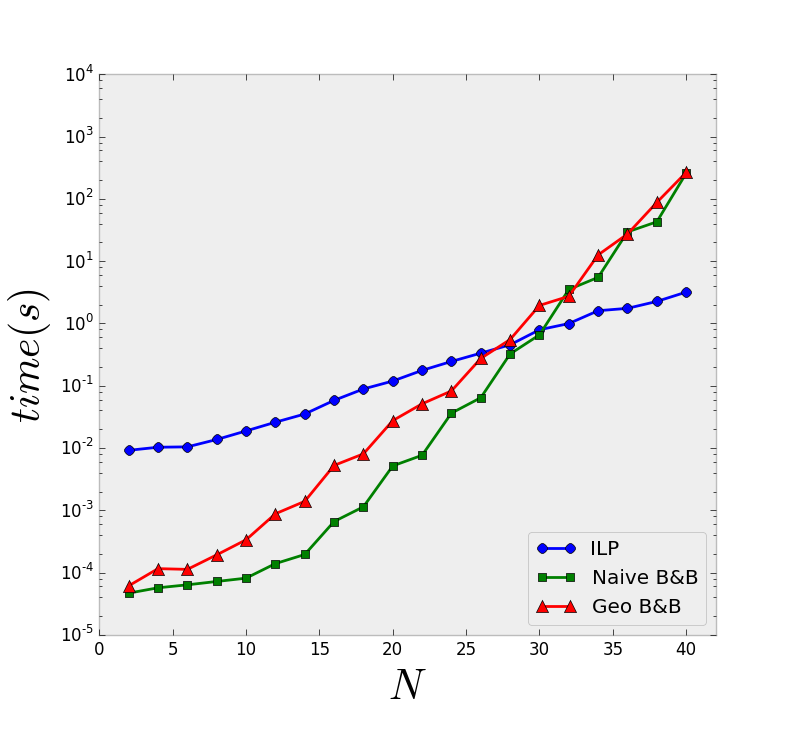
\includegraphics[width=0.9\linewidth]{Pictures/k1} 
		\caption{$K=0.25N$} 
		\label{fig:fixed_k:a} 
	\end{subfigure}%% 
	\begin{subfigure}[b]{0.4\linewidth}
		\centering
		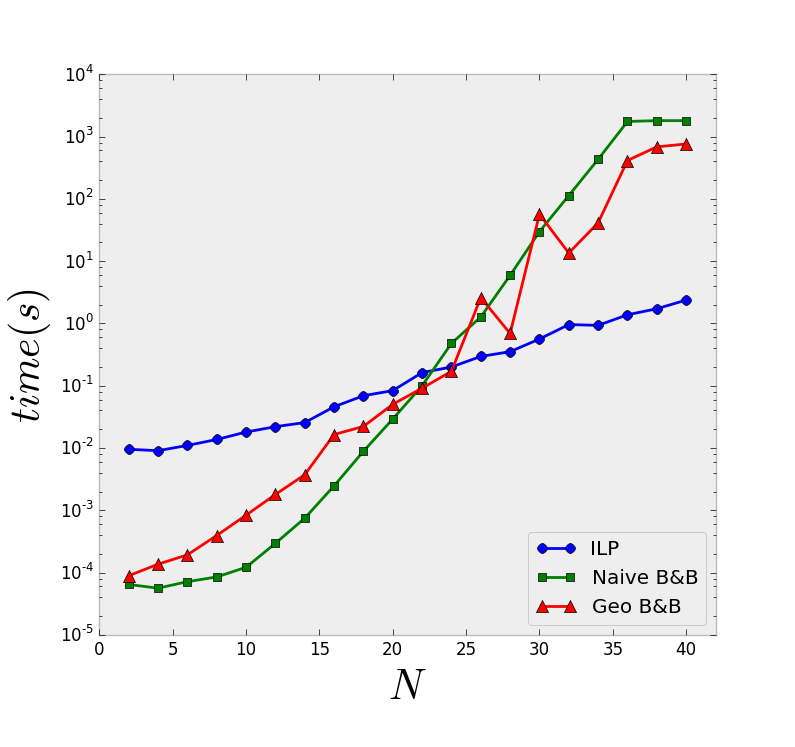
\includegraphics[width=0.9\linewidth]{Pictures/k2} 
		\caption{$K=0.5N$} 
		\label{fig:fixed_k:b} 
	\end{subfigure} 
	\begin{center}
	\begin{subfigure}[b]{0.4\linewidth}
		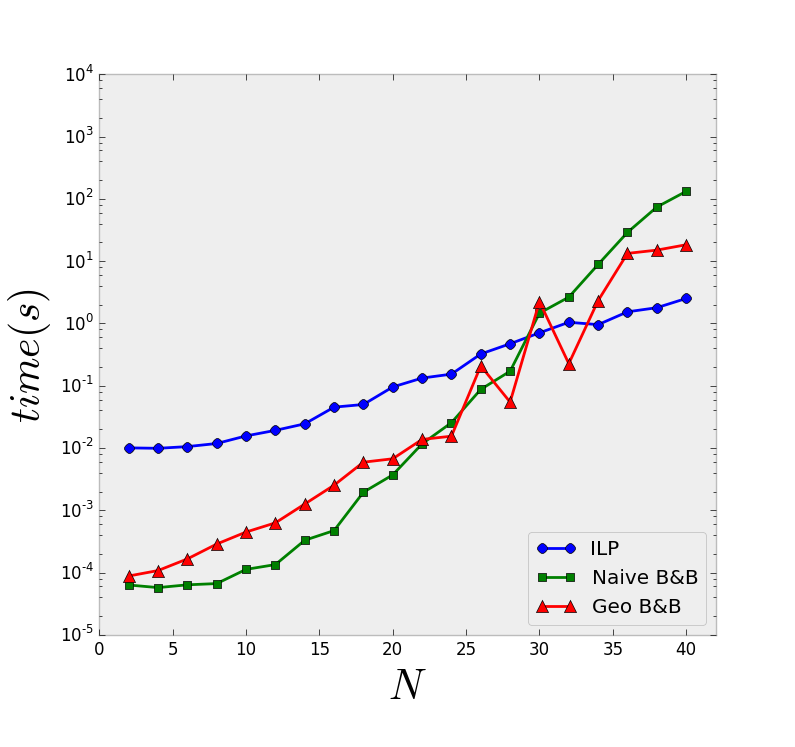
\includegraphics[width=0.9\linewidth]{Pictures/k3} 
		\caption{$K=0.75N$} 
		\label{fig:fixed_k:c} 
	\end{subfigure}
	\end{center}
	\begin{center}
    \textcolor{blue}{\cmark}\ -- Integer Linear Programming\quad   \textcolor{red}{\tmark}\ -- Delaunay Assisted B\&B\quad \textcolor{green}{\smark}\ -- Naive B\&B
    \end{center}
	\caption{CPU-time for different values of $K$ with varying values of $N$}
	\label{fig:fixed_k} 
\end{figure}

		
}
\frame{
	\frametitle{Algorithm Comparison}
	\begin{figure}[t] 
  \begin{subfigure}[b]{0.5\linewidth}
    \centering
    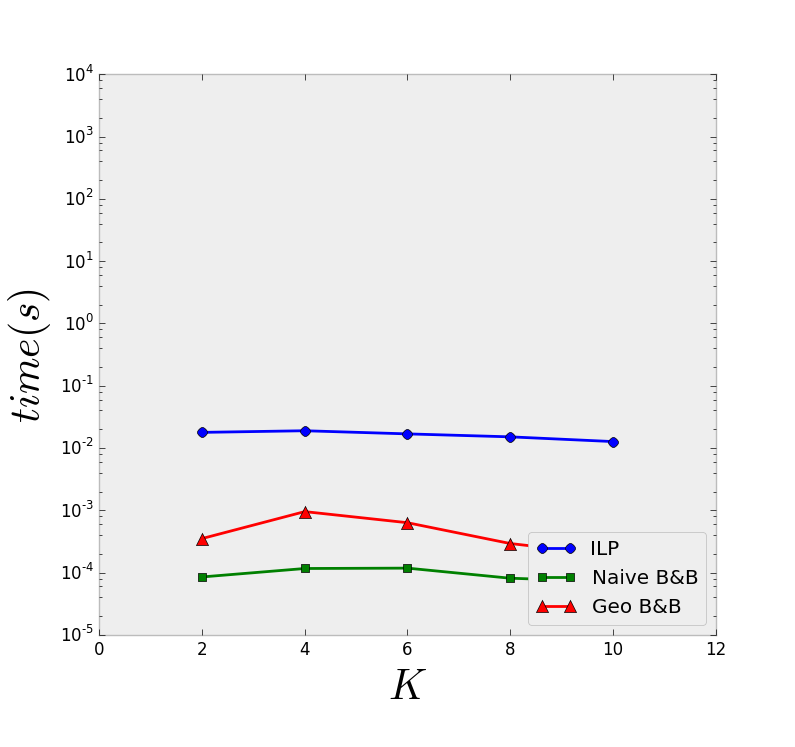
\includegraphics[width=0.9\linewidth]{Pictures/n10} 
    \caption{$N=10$} 
    \label{fig:fixed_n:a} 
    \vspace{4ex}
  \end{subfigure}%% 
  \begin{subfigure}[b]{0.5\linewidth}
    \centering
    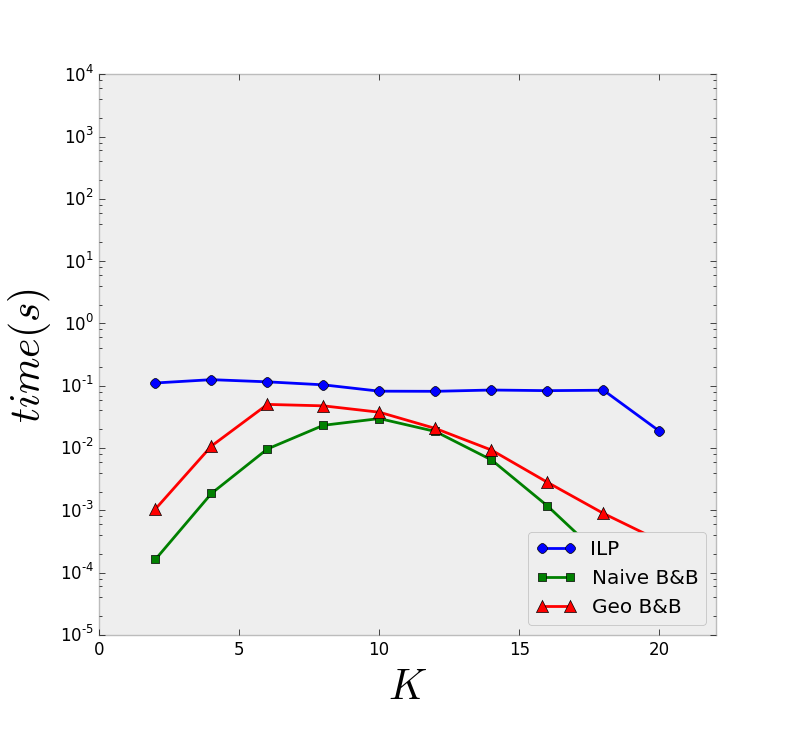
\includegraphics[width=0.9\linewidth]{Pictures/n20} 
    \caption{$N=20$} 
    \label{fig:fixed_n:b} 
    \vspace{4ex}
  \end{subfigure} 
  \begin{subfigure}[b]{0.5\linewidth}
    \centering
    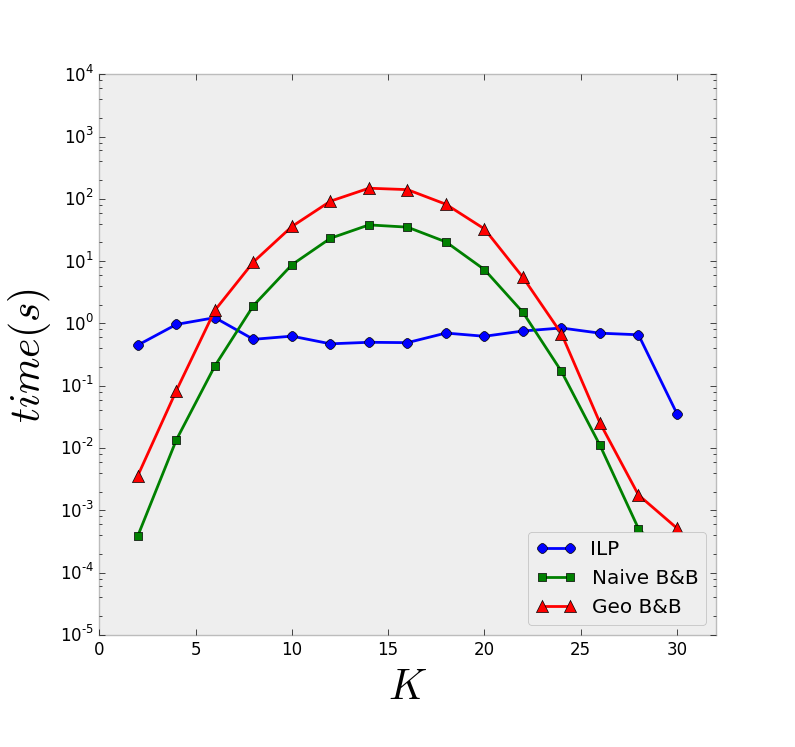
\includegraphics[width=0.9\linewidth]{Pictures/n30} 
    \caption{$N=30$} 
    \label{fig:fixed_n:c} 
  \end{subfigure}%%
  \begin{subfigure}[b]{0.5\linewidth}
    \centering
    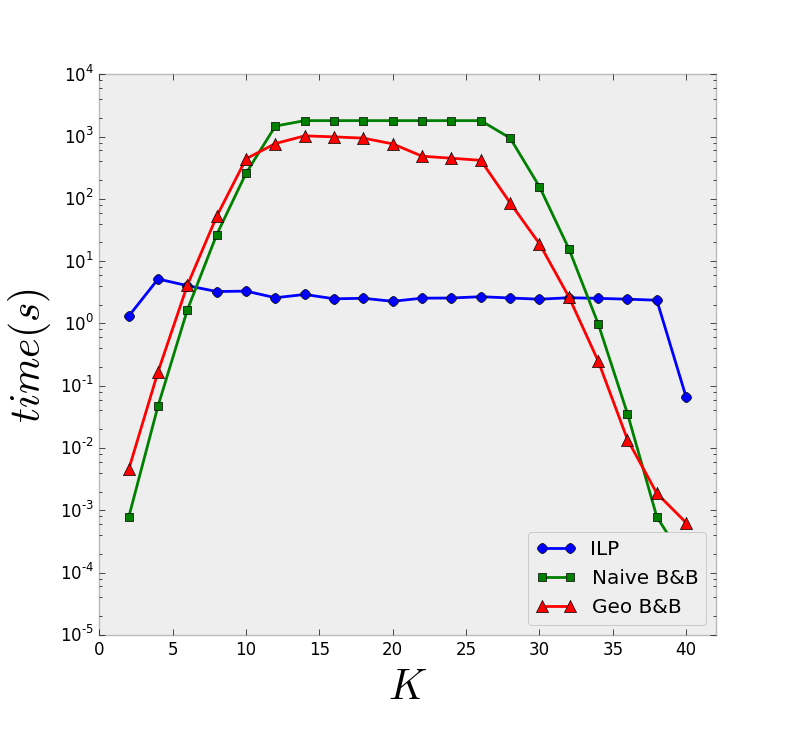
\includegraphics[width=0.9\linewidth]{Pictures/n40} 
    \caption{$N=40$} 
    \label{fig:fixed_n:d} 
  \end{subfigure} 
  \vspace{2ex}
  \begin{center}
  \textcolor{blue}{\cmark}\ -- Integer Linear Programming \quad   \textcolor{red}{\tmark}\ -- Delaunay Assisted B\&B\quad \textcolor{OliveGreen}{\smark}\ -- Naive B\&B
  \end{center}
  \caption{CPU-time for different values of $N$ with varying $K$}
  \label{fig:fixed_n} 
\end{figure}

		
}

\frame{
	\frametitle{Future Work}
	\begin{itemize}
		\item Integration with WFS standard
		\item Heuristic Approach
		\item Approximation Algorithms
		\item Benchmark with real data
	\end{itemize}
}

\end{document}
